%%%% ijcai21.tex

% These are the instructions for authors for IJCAI-21.

\documentclass{article}
\pdfpagewidth=8.5in
\pdfpageheight=11in
% The file ijcai21.sty is NOT the same than previous years'
\usepackage{ijcai21}

% Use the postscript times font!
\usepackage{times}
\usepackage{soul}
\usepackage{url}
\usepackage[hidelinks]{hyperref}
\usepackage[utf8]{inputenc}
\usepackage[small]{caption}
\usepackage{graphicx}
\usepackage{amsmath,amssymb}
\usepackage{amsthm}
\usepackage{booktabs}
% \usepackage{natbib}
% \usepackage{algorithm}
% \usepackage{algorithmic}
\urlstyle{same}
\newcommand\citet[1]{\citeauthor{#1}~[\citeyear{#1}]}


\usepackage[dvipsnames]{xcolor}
\usepackage[ruled,linesnumbered]{algorithm2e}
% \usepackage{color (if used in text)
\usepackage{xspace} 
% the following package is optional:
%\usepackage{latexsym}
\usepackage{paralist}
\setdefaultenum{\bfseries(i)}{}{}{}

\usepackage[normalem]{ulem}

\newcommand\m[1]{\ensuremath{\mathcal{#1}}}
\newcommand\ignore[1]{}
\usepackage[capitalise]{cleveref}
\newcommand\comment[1]{\marginpar{\parbox{\marginparwidth}{\tiny #1}}}
\renewcommand\comment[1]{#1}
% uncomment this for disabling all comments
% \renewcommand\comment[1]{}
\newcommand{\tias}[1]{{\comment{\color{blue}\textsc{TG:}#1}}}
\newcommand{\emilio}[1]{{\comment{\color{orange}\textsc{EG:}#1}}}
\newcommand{\bart}[1]{{\comment{\color{OliveGreen}\textsc{BB:}#1}}}
\newcommand{\todo}[1]{{\comment{\color{red}\textsc{TODO:}#1} }}
\newcommand\voc{\ensuremath{\Sigma}\xspace}
% \newtheorem{definition}{Definition}
% \newtheorem{proposition}{Proposition}
% \newtheorem{lemma}{Lemma}
% \newtheorem{example}{Example}

\newtheorem{thm}{Theorem}
\newtheorem{definition}[thm]{Definition}
\newtheorem{prop}{Property} 
\newtheorem{property}[prop]{Property}
\newtheorem{lem}{Lemma}
\newtheorem{lemma}[lem]{Lemma}
\newtheorem{proposition}[thm]{Proposition} 
\newtheorem{theorem}[thm]{Theorem}
\newtheorem{ex}{Example}
\newtheorem{example}[ex]{Example}

\newcommand\muses[1]{\ensuremath{\mathit{MUSs}(#1)}\xspace}
\newcommand\mcses[1]{\ensuremath{\mathit{MCSs}(#1)}\xspace}

% \newcommand\setstohit{\ensuremath{\m{H} }\xspace}
% \newcommand\setstohitall{\ensuremath{\m{H}_\mathit{all} }\xspace}
% \newcommand\formula{\ensuremath{\m{F} }\xspace}
% \newcommand\formulac{\ensuremath{\m{C} }\xspace}
% \newcommand\formulag{\ensuremath{\m{G} }\xspace}
% \newcommand\mm[1]{\ensuremath{#1}\xspace} 
% \newcommand\nat{\mm{\mathbb{N}}}
% \newcommand\ltrue{\mm{\textbf{t}}}
% \newcommand\lfalse{\mm{\textbf{f}}}

% \newcommand\call[1]{\mm{\textsc{#1}}}
% \newcommand\geths{\mm{\call{GetHittingSet}}}
% \newcommand\ohs{\mm{\call{OptHittingSet}}}
% \newcommand\ghs{\mm{\call{GreedyHittingSet}}}
% \newcommand\ihs{\mm{\call{IncrementalHittingSet}}}
% \newcommand\cohs{\mm{\call{CondOptHittingSet}}}
% \newcommand\sat{\mm{\call{sat}}}
% \newcommand\grow{\mm{\call{Grow}}}
% \newcommand\omus{\mm{\call{OUS}}}
% \newcommand\comus{\mm{\call{c-OUS}}}
% \newcommand\omusinc{\mm{\call{OUS-Inc}}}
% \newcommand\store{\mm{\call{Store}}}
% \newcommand\optprop{\mm{\call{OptimalPropagate}}}
% \newcommand\hitsetbased{hitting set--based\xspace} %en-dash!


\newcommand\setstohit{\ensuremath{\m{H} }\xspace}
\newcommand\F{\ensuremath{\m{F} }\xspace}
% \newcommand\ohs{\ensuremath{\m{OHS} }\xspace}
\newcommand\setstohitall{\ensuremath{\m{H}_\mathit{all} }\xspace}
\newcommand\Iend{\ensuremath{I_\mathit{end} }\xspace}
\newcommand\formula{\ensuremath{\m{F} }\xspace}
\newcommand\formulac{\ensuremath{\m{C} }\xspace}
\newcommand\formulag{\ensuremath{\m{G} }\xspace}
\newcommand\mm[1]{\ensuremath{#1}\xspace}
\newcommand\nat{\mm{\mathbb{N}}}
\newcommand\ltrue{\mm{\textbf{t}}}
\newcommand\lfalse{\mm{\textbf{f}}}
\newcommand\uservars{\ensuremath{\m{U} }\xspace}

\newcommand\satsets{\mm{\mathbf{SSs}}}
\newcommand\fall{\mm{\formula_{\mathit{all}}}}

\newcommand\call[1]{\mm{\textsc{#1}}}
\newcommand\geths{\mm{\call{GetHittingSet}}}
\newcommand\ohs{\mm{\call{OptHittingSet}}}
\newcommand\ghs{\mm{\call{GreedyHittingSet}}}
\newcommand\ihs{\mm{\call{IncrementalHittingSet}}}
\newcommand\cohs{\mm{\call{CondOptHittingSet}}}
\newcommand\chs{\mm{\call{CondHittingSet}}}
\newcommand\sat{\mm{\call{sat}}}
\newcommand\grow{\mm{\call{Grow}}}
\newcommand\omus{\mm{\call{OUS}}}
\newcommand\comus{\mm{\call{OCUS}}}
\newcommand\omusinc{\mm{\call{OUS-Inc}}}
\newcommand\store{\mm{\call{Store}}}
\newcommand\optprop{\mm{\call{MaxConsequence}}}
\newcommand\initsat{\mm{\call{InitSat}}}
\newcommand\hitsetbased{hitting set--based\xspace} %en-dash!
% \newcommand\fall{\mm{\formula_{\mathit{all}}}}
\newcommand\algemilio[1]{\emilio{#1}\;}
% \usepackage[capitalize]{cleveref}

% \call{}
% \usepackage{amsthm}

%REDUCE BIB SIZE                                                                                                                                                        
\let\OLDthebibliography\thebibliography
\renewcommand\thebibliography[1]{
\OLDthebibliography{#1}
\setlength{\parskip}{0pt}                                                                                                                                                \setlength{\itemsep}{0pt}                                                                                                                                              }                                                                                                                                                                             

\SetKwInOut{Input}{Input}
\SetKwInOut{OptInput}{Optional}
\SetKwInOut{Output}{Output}
\SetKwInOut{State}{State}
\SetKwInOut{Ext.}{Ext}
\SetKwComment{command}{/*}{*/}


\newcommand\negset[1]{\mm{\overline{#1}}}
% \newcommand\Iend{\mm{I_{\mathit{end}}}}
\newcommand\maxsat{MaxSAT\xspace}

%PDF Info Is REQUIRED.
\pdfinfo{
/Title (Incremental and Constrained Optimal Unsatisfiable Subsets for Explaining CSPs)
/Author (Anyonymous)
/TemplateVersion (IJCAI.2021.0)
}

% \title{Incremental and Constrained Optimal Unsatisfiable Subsets for Explaining CSPs}
% \title{Constrained Optimal Unsatisfiable Subsets for Explaining CSPs}
\title{Efficiently Explaining CSPs with Unsatisfiable Subset Optimization}

% Single author syntax
\author{Anonymous}

\usepackage{etoolbox}

\newcommand\setcitation[2]{%
  \csdef{mycommoncitation#1}{#2}}
\newcommand\getcitation[1]{%
  \csuse{mycommoncitation#1}}

\setcitation{IDP}{WarrenBook/DeCatBBD14}
\setcitation{idp}{WarrenBook/DeCatBBD14}
\setcitation{fodot}{tocl/DeneckerT08}
\setcitation{foid}{tocl/DeneckerT08}
\setcitation{FOID}{tocl/DeneckerT08}
\setcitation{cplogic}{journal/tplp/VennekensDB10}
\setcitation{CPlogic}{journal/tplp/VennekensDB10}
\setcitation{CPLogic}{journal/tplp/VennekensDB10}
\setcitation{CP}{fai/Rossi06}
\setcitation{cp}{fai/Rossi06}
\setcitation{EZCSP}{lpnmr/Balduccini11}
\setcitation{KR}{Baral:2003}
\setcitation{ASPComp2}{lpnmr/DeneckerVBGT09}
\setcitation{ASPComp3}{journals/tplp/CalimeriIR14}
\setcitation{ASPComp4}{conf/lpnmr/AlvianoCCDDIKKOPPRRSSSWX13}
\setcitation{ASPComp5}{journals/ai/CalimeriGMR16}
\setcitation{ASPComp6}{jair/GebserMR17}
\setcitation{ASPComp7}{tplp/GebserMR20}
\setcitation{CPSupport}{ictai/DeCat13}
\setcitation{CPsupport}{ictai/DeCat13}
\setcitation{functionDetection}{iclp/DeCatB13}
\setcitation{FunctionDetection}{iclp/DeCatB13}
\setcitation{fodot2asp}{DeneckerLTV12} %TODO replace by journal publication if one is publishedr
\setcitation{Tarskian}{DeneckerLTV12} %Same as the one above 
\setcitation{TarskianSemanticsASP}{DeneckerLTV12} %Same as the one above 
\setcitation{Inca}{iclp/DrescherW12}
\setcitation{csp2asp}{ijcai/DrescherW11}
\setcitation{DPLLT}{cav/GanzingerHNOT04}
\setcitation{AspInPractice}{synthesis/2012Gebser}
\setcitation{ASPInPractice}{synthesis/2012Gebser}
\setcitation{clasp}{ai/GebserKS12}
\setcitation{oclingo}{kr/GebserGKOSS12}
\setcitation{clingo}{iclp/GebserKKOSW16}
\setcitation{gringo}{lpnmr/GebserST07}
\setcitation{cmodels}{aaai/GiunchigliaLM04}
\setcitation{inputster}{tplp/Jansen13}
\setcitation{DLV}{tocl/LeonePFEGPS06}
\setcitation{LearningPaper}{TPLP/BruynoogheBBDDJLRDV} %TODO replace by published version
\setcitation{clog}{iclp/BogaertsVDV14} %TODO replace by journal publication if one is published
\setcitation{foc}{iclp/BogaertsVDV14}
\setcitation{FOC}{iclp/BogaertsVDV14}
\setcitation{inferenceClog}{ecai/BogaertsVDV14}
\setcitation{examplesClog}{nmr/BogaertsVDV14b} %TODO replace by better publication if possible
\setcitation{AFT}{DeneckerMT00}
\setcitation{KBS}{iclp/DeneckerV08}
\setcitation{KBS-invitedtalk}{jelia/Denecker16}
\setcitation{KBPE}{inap/DePooterWD11}
\setcitation{lazyGrounding}{jair/CatDBS15} 
\setcitation{LazyGrounding}{jair/CatDBS15} 
\setcitation{lazygrounding}{jair/CatDBS15} 
\setcitation{lazygroundingASP}{ijcai/BogaertsW18} 
\setcitation{justifications}{lpnmr/DeneckerBS15} 
\setcitation{justificationsAlpha}{ijcai/BogaertsW18} 
\setcitation{ASP}{marek99stable}
\setcitation{satid}{sat/MarienWDB08}
\setcitation{lazyclausegeneration}{constraints/OhrimenkoSC09}
\setcitation{FP}{ACMCS/Hudak89}
\setcitation{GroundingWithBounds}{jair/WittocxMD10}
\setcitation{GroundWithBounds}{jair/WittocxMD10}
\setcitation{SAT}{faia/SilvaLM09}
\setcitation{HandbookOfSAT}{faia/2009-185}
\setcitation{LTC}{iclp/Bogaerts14}
\setcitation{SPSAT}{ictai/DevriendtBMDD12}
\setcitation{BreakID}{sat/DevriendtBBD16}
\setcitation{breakid}{sat/DevriendtBBD16}
\setcitation{LCG}{stuckeyLCG}
\setcitation{MiniZinc}{conf/cp/NethercoteSBBDT07}
\setcitation{minizinc}{conf/cp/NethercoteSBBDT07}
\setcitation{amadini}{cpaior/AmadiniGM13}
\setcitation{bootstrapping}{ngc/BogaertsJDJBD16}
\setcitation{Bootstrapping}{ngc/BogaertsJDJBD16}
\setcitation{GroundedFixpoints}{ai/BogaertsVD15}
\setcitation{PartialGroundedFixpoints}{ijcai/BogaertsVD15}
\setcitation{LogicBlox}{datalog/GreenAK12}
\setcitation{proB}{journals/sttt/LeuschelB08}
\setcitation{NaturalInductions}{KR/DeneckerV14} %TODO replace by journal publication if one is published
\setcitation{LP}{jacm/EmdenK76}
\setcitation{SMT}{faia/BarrettSST09}
\setcitation{AF}{ai/Dung95}
\setcitation{ADF}{kr/BrewkaW10}
\setcitation{af}{ai/Dung95}
\setcitation{adf}{kr/BrewkaW10}
\setcitation{ADFRevisited}{ijcai/BrewkaSEWW13}
\setcitation{adfrevisited}{ijcai/BrewkaSEWW13}
\setcitation{DefaultLogic}{ai/Reiter80}
\setcitation{DL}{ai/Reiter80}
\setcitation{AEL}{mo85}
\setcitation{minisat}{sat/EenS03}
\setcitation{completion}{adbt/Clark78}
\setcitation{ClarkCompletion}{adbt/Clark78}
\setcitation{wasp}{lpnmr/AlvianoDFLR13}
\setcitation{minisatid}{ictai/DeCat13}
\setcitation{lcg}{stuckeyLCG}
\setcitation{CEGAR}{jacm/ClarkeGJLV03}
\setcitation{cegar}{jacm/ClarkeGJLV03}
\setcitation{CuttingPlane}{or/DantzigFJ54}
\setcitation{kodkod}{tacas/TorlakJ07}
\setcitation{cdcl}{Marques-SilvaS99}
\setcitation{CDCL}{Marques-SilvaS99}
\setcitation{1UIP}{iccad/ZhangMMM01}
\setcitation{relevance}{ijcai/JansenBDJD16}
\setcitation{relevance-implementation}{aspocp/JansenBDJD16}
\setcitation{WFS}{GelderRS91}
\setcitation{wfs}{GelderRS91}
\setcitation{UnfoundedSet}{GelderRS91}
\setcitation{UFS}{GelderRS91}
\setcitation{stablesemantics}{iclp/GelfondL88}
\setcitation{StableSemantics}{iclp/GelfondL88}
\setcitation{shatter}{Shatter}
\setcitation{sbass}{drtiwa11a}
\setcitation{lparsemanual}{url:lparse_manual}
\setcitation{AIC}{ppdp/FlescaGZ04}
\setcitation{templates}{tplp/DassevilleHJD15}
\setcitation{templates2}{iclp/DassevilleHBJD16}
\setcitation{sat-to-sat}{aaai/JanhunenTT16}
\setcitation{sat-to-sat-qbf}{bnp/BogaertsJT16}
\setcitation{sat-to-sat-QBF}{bnp/BogaertsJT16}
\setcitation{sat-to-sat-SO}{kr/BogaertsJT16}
\setcitation{XSB}{SwiW12}
\setcitation{KCmap}{jair/DarwicheM02}
\setcitation{TLA}{DBLP:books/aw/Lamport2002}
\setcitation{EventB}{BookAbrial2010}
\setcitation{MX}{MitchellT05}
\setcitation{MIP}{Sierksma96}
\setcitation{perefectmodel}{minker88/Przymusinski88}
\setcitation{SafeInductions}{ijcai/BogaertsVD17}
\setcitation{AIC}{ppdp/FlescaGZ04}
\setcitation{aic}{ppdp/FlescaGZ04}
\setcitation{alpha}{lpnmr/Weinzierl17}
\setcitation{omiga}{jelia/Dao-TranEFWW12}
\setcitation{gasp}{fuin/PaluDPR09}
\setcitation{asperix}{lpnmr/LefevreN09a}
\setcitation{CTL}{lop/ClarkeE81}
\setcitation{AFT-AIC}{ai/BogaertsC18}
\setcitation{UltimateApproximator}{DeneckerMT04}
\setcitation{KripkeKleene}{Fitting85}
\setcitation{AFT-HO}{corr/CharalambidisRS18} %TODO replace
\setcitation{HereThere}{Heyting30}
\setcitation{dAEL}{ijcai/HertumCBD16}
\setcitation{SDD}{ijcai/Darwiche11}
\setcitation{HEX}{ijcai/EiterIST05}
\setcitation{wADF}{aaai/BrewkaSWW18}
\setcitation{wADFfix}{corr/BrewkaSWW18}
\setcitation{TransitionSystems}{jacm/NieuwenhuisOT06}
\setcitation{galliwasp}{lopstr/MarpleG12}
\setcitation{GalliWasp}{lopstr/MarpleG12}
\setcitation{clingcon}{tplp/BanbaraKOS17}
\setcitation{lp2sat}{birthday/JanhunenN11}
\setcitation{lp2mip}{LIU12}
\setcitation{lp2diff}{lpnmr/JanhunenNS09}
\setcitation{lp2acyc}{ecai/GebserJR14}
\setcitation{PB}{faia/RousselM09}
\setcitation{pb}{faia/RousselM09}
\setcitation{CuttingPlanes}{dam/CookCT87}
\setcitation{RoundingSAT}{ijcai/ElffersN18}
\setcitation{PRS}{aaai/DixonG02}
\setcitation{sat4j}{jsat/BerreP10}
\setcitation{SAT4J}{jsat/BerreP10}
\setcitation{mingo}{LIU12}
\setcitation{pbmodels}{lpnmr/LiuT05}
\setcitation{HEF-LP}{lpnmr/GebserLL07}
\setcitation{HCF-LP}{amai/Ben-EliyahuD94}
\setcitation{aspcore2}{AspCore2}
\setcitation{}{}
\setcitation{}{}
\setcitation{}{}
\setcitation{}{}
\setcitation{}{}
\setcitation{}{}
\setcitation{}{}
\setcitation{}{}
\setcitation{}{}
\setcitation{}{}
\setcitation{}{}
\setcitation{}{}
\setcitation{}{}
\setcitation{}{}
\setcitation{}{}
\setcitation{}{}
\setcitation{}{}
\setcitation{}{}
\setcitation{}{}
\setcitation{}{}
\setcitation{}{}
\setcitation{}{}
\setcitation{}{}
  
 %Command for in case you want multiple citations in one, e.g., \cite{\refto{fodot},\refto{idp}}
 %Warning: no safety checks
\newcommand\refto[1]{%
      \ifcsname mycommoncitation#1\endcsname%
      \getcitation{#1}%
      \else%
      #1%
      \fi%
      }
      
 %usage: \mycite{key}, e.g., \mycite{fodot} results in \cite{tocl/DeneckerT08}
\newcommand\mycite[1]{%
      \ifcsname mycommoncitation#1\endcsname%
   \cite{\getcitation{#1}}%
  \else%
    \cite{#1}%
  \fi%
}	
  
   %usage: \mycite{key}, e.g., \mycite{fodot} results in \cite{tocl/DeneckerT08}
\newcommand\mycitet[1]{%
      \ifcsname mycommoncitation#1\endcsname%
   \citet{\getcitation{#1}}%
  \else%
    \citet{#1}
  \fi%
}	
  


\begin{document}
 
\maketitle

\begin{abstract}
Recently, a novel method for explaining solutions of constraint satisfaction problems was proposed. 
% 
An explanation here is a \textit{sequence} of simple inference steps, where the simplicity of an inference step depends on the number and types of constraints used, eventually explaining all logical consequences of the problem. 
% (I would even drop this: For CSPs that have a unique solution, this corresponds to explaining each decision variable's assignment in that full solution.)
% what?
The current paper %tackles two questions left in 
builds on these formal foundations and tackles two emerging questions: namely how to generate explanations that are provably optimal (with respect to the given cost metric) and how to generate them efficiently. 
% how? 
To answer these questions, we develop 1) an implicit hitting set algorithm for finding \textit{optimal} unsatisfiable subsets; 2) a method to reduce multiple calls for (optimal) unsatisfiable subsets to a single call that takes \emph{constraints} on the subset into account, and 3) a method for re-using relevant information over multiple calls to these algorithms. 
%     This raises the need for algorithms that can compute unsatisfiable subsets of a logical specification that are optimal with respect to a certain cost criterion.
%     We tackle this challenge by developing an algorithm for computing cost-optimal unsatisfiable subsets inspired by minimal hitting set dualization approaches for finding cardinality-minimal unsatisfiable subsets and for solving partial weighted \maxsat.
%     For generating explanations, many subsequent calls for cost-optimal unsatisfiable subsets will be performed on closely related theories.
%     Inspired by this, we show how the hitting set dualization approach allows us to reuse computation results when solving many variations of the same problems.
%     We generalize our approach to a setting that allows for imposing constraints on the structure of the unsatisfiable subsets of interest.
%     We evaluate all our algorithms in the explanation-generation context.
%     % in terms of the runtime and computational feasibility, as well as the quality of the obtained explanation sequence.
We show that this approach can be used to effectively find sequences of \textit{optimal} explanations for constrained satisfaction problems like logic grid puzzles.
\end{abstract}

\section{Introduction}
% \todo{1 - 1 1/2 column} 
% {\color{OliveGreen} OLD TEXT TO BE REWRITTEN
% !TeX root = ./main.tex

% Research

In recent research, a novel method for explaining the inferences made by constraint satisfaction solver was developed \cite{ecai/BogaertsGCG20}. 
While the techniques were developed for explaining satisfiable constraint satisfaction problems, the developed algorithms relied heavily on calls for so-called \emph{Minimal Unsatisfiable Subsets} (MUS), exploiting a one-to-one correspondence between so-called non-redundant explanations and MUSs. 
The algorithm developed by \citet{ecai/BogaertsGCG20} has two weaknesses: first of all, it provides no guarantees about the quality of the produced explanations due to internally computing $\subseteq$-minimal unsatisfiable subsets, which are often suboptimal with respect to the quality of an explanations step. Secondly, it suffers from performance problems: the lack of optimality is partly overcome by replacing a potential single call for a cost-optimal MUS by multiple calls, but this very high number of MUS calls causes that even for simple puzzles for which the unique solution can be found in a fraction of a second, the explanation generation process takes several hours. 


Motivated by these observations, we develop algorithms for MUS optimization (i.e., for computing cost-optimal MUSs) given some cost function. The algorithm we develop take inspiration from 
hitting set--based %The en-dash is on purpose! 
algorithms to compute cardinality-minimal MUSs \cite{ignatiev2015smallest} and for MAXSAT solving \cite{davies}. 

Furthermore, given the fact that a single call for generation of an explanation sequence internally employs several calls OMUS calls for each explanation step, whit all OMUS calls starting from approximately the same theory, we develop \emph{incremental} algorithms that allow reusing as many results as possible from earlier calls, so as to improve the overall runtime. 

We implemented these ideas in the cppy framework \cite{cppy}  and experimentally validate them on the puzzles of \citet{ecai/BogaertsGCG20} as well as on ... 
\todo{To be filled in later}
Our experimental results indicate that
\begin{itemize}
  \item confirm Davies's observations 
  \item show that incrementality is of crucial importance for the explanation generation task
  \item ... 
\end{itemize}
... \todo{To be filled in later} 

Summarized, the main contributions of our paper are:
\begin{itemize}
  \item We generalize the algorithm of \citet{} to allow for arbitrary \emph{monotonic} (with respect to set inclusion) optimization functions
  \item We extend by translating techniques developed for maxsat \cite{davies} and exploiting them for MUS search
  \item We develop techniques for reusing parts of the computations of an OMUS call in future OMUS calls, thereby essentially developing the first incremental OMUS solver. 
  \item We experimentally validate our algorithms in the explanation generation context of \citet{}
\end{itemize}



% the very many MUS calls have as a consequence that 
\emilio{Rephrase Intro: In the last few years, as AI systems employ more advanced reasoning mechanisms and computation power, it becomes increasingly difficult to understand why certain decisions are made.
Explainable (XAI), a subfield of AI, aims to fulfil the need for trustworthy AI systems to understand \emph{how} and \emph{why} the system made a decision, e.g. for verifying correctness of the system, as well as to control for biased or systematically unfair decisions.

Despite the fact that we do not (specifically) aim to explain over-constrained problems, our algorithms will also internally make use of methods to extract a minimal set of conflicting constraints often called a \emph{\underline{M}inimal \underline{U}nsatisfiable \underline{S}ubset} (MUS) or \emph{Minimal Unsatisfiable Core} \cite{marques2010minimal}.

While explainability of constraint optimisation has received little attention so far, in the related field of \textit{planning}, there is the emerging subfield of \textit{eXplainable AI planning} (XAIP)~\cite{fox2017explainable}, which is concerned with building planning systems that can explain their own behaviour.
This includes answering queries such as ``why did the system (not) make a certain decision?'', ``why is this the best decision?'', etc. In contrast to explainable machine learning research~\cite{guidotti2018survey}, in explainable planning one can make use of the explicit \textit{model-based representation} over which the reasoning happens.
Likewise, we will make use of the constraint specification available to constraint solvers, more specifically typed first-order logic~\cite{atcl/Wittocx13}.

This research fits within the general topic of Explainable Agency~\cite{langley2017explainable}, whereby in order for people to trust autonomous agents, the latter must be able to \textit{explain their decisions} and the \textit{reasoning} that produced their choices.
To provide the constraint solver with Explainable Agency~\cite{langley2017explainable}, we first formalize the problem of step-wise explaining the propagation of a constraint solver through a sequence of small inference steps.
Next, we use an optimistic estimate of a given cost function quantifying human interpretability to guide the search to \textit{simple}, low-cost, explanations thereby making use of minimal unsatisfiable subsets.
We extend this approach using \emph{reasoning by contradiction} to produce additional explanations of still difficult-to-understand inference steps.
Finally, we discuss the challenges and some outlooks to explaining how to solve constraint satisfaction problems.


\paragraph*{Publication history} This workshop paper is an extended abstract of previous papers presented at workshops and conferences \cite{claesuser,DBLP:conf/bnaic/ClaesBCGG19,ecai/BogaertsGCG20} and a journal paper under review \cite{bogaerts2020framework}.
}

\begin{enumerate}
    \item XAI
    \item MUS vs Overconstrained/Infeasibility
    \item CSP
    \item XOPT
\end{enumerate}

Contributions : 
\begin{enumerate}
    \item Efficient, greedy algorithm for explaining CSP based on OMUS 
    \item Adapatation smallest MUS adaptation to OMUS (different hs + no maxsat) 
    \item Improving OMUS algorithm from Davies' related delayed MaxSAT algorithm 
    \item Incremental OMUS computation to speed-up explanations
    \begin{itemize}
        \item hoe belangrijk is de incrementaliteit in het algorithme
        \item kunnen  we nog meer incrementeel verder gaan
    \end{itemize}
    \todo{
    \begin{itemize}
        \item Bestaande SMUS/OMUS algorihtmes incrementeel veranderen
        \begin{itemize}
            \item Bredere studie, SMUS => OMUS veralgemenen
            \item Hoe efficient zijn ze om ons probleem op te lossen
        \end{itemize}
    \end{itemize}
    }
\end{enumerate}


% }

\section{Background}\label{sec:backgr}\label{sec:background}
% \todo{1 1/2 -2 columns}
% !TeX root = ./main.tex

In this section, we discuss background on the hitting set duality, which constitutes the core of our algorithm. 
We present all result using propositional logic  as a representation language, as is common in hitting set--based approaches, but the algorithm works equally well for other languages with a model semantics. 
 
%  
% 
% 
% The overarching goal of this paper is to generate a sequence of small reasoning steps, each with an interpretable explanation, and for that we introduce the necessary background.
% \begin{itemize}
%     \item Explanation sequence : CSP journal paper ?
%     \item concept of OMUS
%     % \item Logic grid puzzles (depends on experiments)
%     % \item Nested explanation still applicable?
% \end{itemize}

\newcommand\F{\m{F}}
Let \voc be a set of propositional symbols, also called \emph{atoms}; this set is implicit in the rest of the paper. A \emph{literal} is an atom $p$ or its negation $\lnot p$. A clause is a disjunction of literals. A formula $\m{F}$ is a conjunction of clauses. 
Slightly abusing notation, a clause is sometimes used as a set of literals and a formula as a set of clauses.
% \todo{weight function comes later}
A \emph{weight function} $w$ on $\m{F}$ assigns to each clause in $\m{F}$ either a positive integer, or a $\infty$. 
A \emph{model} is a truth assignment
 to the atoms that satisfies $\m{F}$.
$\m{F}$ is said to be \emph{unsatisfiable} if it has no models. 

\begin{definition}
  A \emph{Minimal Unsatisfiable Subset} (MUS) of \F is a set $\m{S} \subseteq \F$  that is unsatisfiable but such that every strict subset of $\m{S} $ is satisfiable. 
%   
  We write \muses{\F} for the set of MUSs of \F. 
\end{definition}


% Formally, we define a \textit{Minimum Unsatisfiable Subset} (MUS), as a set of clauses that taken together are unsatisfiable, but if any of the clauses are removed then the reduced formula becomes satisfiable.

\begin{definition}
    A set $\m{S} \subseteq \m{F}$ is a \emph{Maximal Satisfiable Subset} (MSS) of $ \m{F}$ if $\m{S}$ is satisfiable and for all $\m{S}'$ with $\m{S}  \subsetneq  \m{S}'\subseteq\m{F} $, $\m{S}'$ is unsatisfiable.
\end{definition}

\begin{definition}
    A subset $\m{C} \subseteq \m{F}$ is a \emph{Minimal Correction Subset} (MCS) if $\m{F}\setminus\m{C}$ is satisfiable, while for all 
    $ \m{C}' \subsetneq C$,  $\m{F} \setminus \m{C}'$ is unsatisfiable.
    We write \mcses{\F} for the set of MCSs of \F. 
\end{definition}

It is well-known that if $\m{F}$ is unsatisfiable, each  MCS is the complement of an MSS and vice versa. 

\begin{definition}\label{def:minimal-hs}
    Given a collection of sets $\m{K}$, a hitting set $h$ is a set such that $\forall \ C \in \m{K}$, $h \cap C \neq \emptyset$. A hitting set is \emph{minimal} if no strict subset of it is also a hitting set. 
\end{definition}

% \noindent In fact, for a collection of sets $\m{K}$ there exist multiple possible minimal hitting sets on $\m{K}$. Consequently, we define the \textbf{minimum} hitting set as:

% \begin{definition}\label{def:minimum-hs}
% %     Let $\m{K}$ be a collection of sets and $HS(\m{K})$ be the collection of all minimal hitting sets on $\m{K}$.
% %     A hitting set $hs$ is a \textbf{minimum} hitting set if $\forall \ h' \in HS(\m{K}): |hs| \leq |h'|$.
%   \end{definition}

The following proposition is the well-known hitting set duality  between MCSs and MUSs that forms the basis of our algorithms \cite{DBLP:journals/jar/LiffitonS08,ai/Reiter87}.

\begin{proposition}\label{prop:MCS-MUS-hittingset}
%     Given an $ \m{F}$, let MUSes($\m{F}$), be the Minimal Unsatisfiable Subsets of F and MCSes($\m{F}$), be the Minimal Correction Subsets of F:
%     
    A set  $\m{C} \subseteq \m{F}$ is an MCS of $ \m{F}$ iff  $\m{C}$ is a \emph{minimal hitting set} of \muses{F}.

    A set  $\m{U} \subseteq \m{F}$ is a MUS of $ \m{F}$ iff  $\m{U}$ is a \emph{minimal hitting set} of \mcses{F}.
\end{proposition}

The duality of proposition \ref{prop:MCS-MUS-hittingset} is fundamental to explaining how we can compute the SMUS in section \ref{sec:smus}. 
% TODO: add something here ?
In section \ref{sec:omus}, we further exploit this proposition for computing the OMUS for a given unsatisfiable CNF formula $\m{F}$.


\section{Motivation}\label{sec:motivation}\label{sec:motviation}
% \todo{The idea of explanation generation, the issues with it, formal}
Our work is motivated by the problem of explaining satisfaction problems through a sequence of simple explanation steps. This can be used to teach people problem-solving skills, to compare the difficulty of related satisfaction problems (through the number and complexity of steps needed), and in human-computer solving assistants.

%\ignore{
%
%\paragraph{Using Constraints to Encode Domain Knowledge}
%
%% {\color{OliveGreen} OLD TEXT TO BE REWRITTEN
%\bart{Not efficient -> Begin paper zeggen. }
%The constraints on OCUSs can not only be used to restrict the set of solutions, but also to improve the solver performance by encoding domain knowledge.
%Indeed, if we know that all ``good'' OCUSs will satisfy certain constraints, or if we know that it suffices to search for OCUSs satisfying certain constraints (because each OCUS can easily be extended to one such OCUS),  we can also encode that knowledge in $p$, thereby restricting the possible options of the hitting set solver, aiming to improve overall performance of the algorithm. 
%
%In the explanation application, we encountered this phenomenon as follows. 
%The clues to be used in explanations were high-level (first-order) constraints. They were translated into clauses, using among other, a Tseitin transformation.
%Hence, in the end the transformation of a single high-level clue consists of several clauses, of which some are definitions of newly introduced variables. 
%Now, the associated cost function was only concerned with the issue ``\emph{was a certain clue used or not?}'', which translates at the lower level to ``\emph{does the OCUS contain at least one clause from the translation of the clue?}''.
%Using such a cost function means that to compute the cost of an OCUS, it does not matter if a single, or if all clauses corresponding to a given clue are used. As such, we might as well include all of them, which can be encoded in $p$ as well.  
%
%An alternative view on the same property is that we can \emph{reify} the high level constraint by considering an indicator variable defining satisfaction of the entire constraint. 
%We can then add the property to $p$ that all reified constraints are \emph{hard constraints}, in the sense that they have to be included in each OCUS (and thus each hitting set). With that, only the truth/falsity of the single indicator variable is considered to be a clause of $\formulac$ that can be enabled/disabled by the hitting set algorithm. 
%% This variable then represent whether or not the high level constraint is active.
%It is easy to see that there is a one to one correspondence between the OCUSs produced by the two approaches. In our implementation, we opted for the latter because of its simplicity. 
%%\tias{is this really to $p$? higher up we argued that we push $p$ into the MIP, but all hard clauses are kept outside of the MIP... I guess saying that har dlcauses are 'always included' is somehow doing that? it also means they are 'constant' in the MIP objective and hence can be removed from it, that is perhaps a more pragmatic view on it...}
%%\emilio{phrases are loooong.}
%}
%<<<<<<< HEAD
%The recent algorithm of ~\citet{ecai/BogaertsGCG20} starts from a formula $\formulac$ (in the application coming from a high level CSP), a partial interpretation $I$ (a conjunction of literals) and a cost function $f$ quantifying the difficulty of an explanation step, by means of a weight for every clause and literal in \formula. % and a set $U$ of atoms whose literals need explaining (e.g., not containing auxiliary variables). 
%=======
Our original explanation generation algorithm \cite{ecai/BogaertsGCG20} starts from a formula $\formulac$ (in the application coming from a high level CSP), a partial interpretation $I$ (here also viewed as a conjunction of literals) and a cost function $f$ quantifying the difficulty of an explanation step, by means of a weight for every clause and literal in \formula. % and a set $U$ of atoms whose literals need explaining (e.g., not containing auxiliary variables). 
%>>>>>>> e1b04e34e56f697a0fa77777308f90e822416410
% \emilio{not sure why we talk about U and not later in the text. U is especially useful with the call to the optimal propagate}
% U not needed, auxiliaries get zero weight then done...

%; more specifically the cautious consequence of $\formulac \wedge I$ projected onto $U$.
 % Not part of input. It is what the algorithm 
%A single explanation step is an inference step $I' \implies N$ where $I' \subseteq I$ and $atoms(I') \subseteq U$.
%\ignore{
%\tias{Optional, alg can move to Apdx:} \cref{alg:explainCSPReal} shows the basic explanation sequence generation algorithm of~\cite{ecai/BogaertsGCG20}. 
%\bart{If it stays, it needs a lot more explaining. For instance the magic going on in lines such as 
%\[       N \gets  (\Iend \setminus I) \cap \optprop(X \cap I).\] 
%A reader cannot understand this. Options are: drop or explain, but definitely not keep just like that.
%
%The way it is currently phrased is also assuming that all the $\formulac$ are \textbf{HARD} constraints. But that is not how Bogaerts et al did it. I would definitely avoid phrasing it that way here because then we have to explain *everything*. That also does not match the OneStep description. 
%So, if it stays, needs to be cleaned-up and made consistent throughtout hte paper and more details are needed. }
%
%
%
%
%
%\begin{algorithm}[t]
%    %\Input{${\cal C}$,  \textit{a CNF ${\cal C}$ over a vocabulary $V$} }
%    %\Input{$U$, \textit{a user vocabulary $U \subseteq V$} }
%    %\Input{$f$, \textit{a cost function $f : 2^{lits({U})} \rightarrow  \mathbb{N} $.}}
%    %\Input{$I$, \textit{a partial interpretation over $U$}}
%    %\Output{$E$, \textit{a sequence of explanation steps as implications $I_{expl} \implies N_{expl}$}}
%    % \vspace*{0.01cm}
%    \DontPrintSemicolon
%    \caption{$\call{ExplainCSP}(\formulac, f, I, U)$}
%    \label{alg:explainCSP}\label{alg:explainCSPReal}
%    %$\sat \gets \initsat({\cal C}$) \;
%        % \tcp{Hyp: f}
%    $I_{end} \gets U \cap \optprop(\formulac \wedge I)$ \;
%    $E \gets \langle \rangle$\;
%    %$U \gets U \cap I_{end}$ \;
%    %$I_{expl} = \{i \in I_{end} | f(i) < inf \wedge f(-i) < inf\}$ \;
%    % \algemilio{bart: What's a better way to get the initial interpr.?}
%    % $I \gets \{l \in I_{end} | f(\lnot l) = inf\}$ \;
%    \While{$(I \cap U) \neq I_{end}$}{
%        %$E \gets \call{bestStep}({\cal C},U, f,\Iend, I)$\;
%        $X \gets \onestep({\cal C},f,I,\Iend)$\;
%        %$I_{\mathit{best}} \gets I \cap X$\;
%        %$\formulac_{\mathit{best}}\gets \formulac\cap X$\;
%        $N \gets  (\Iend \setminus I) \cap \optprop(X \cap I)$\;
%        %add $\{I_{\mathit{best}} \wedge \formulac_{\mathit{best}} \implies N_{\mathit{best}}\}$ to $E$\;
%        add $\{(X \cap I) \implies N\}$ to $E$\;
%        $I \gets I \cup N$\;
%    }
%    \Return{E}\;
%\end{algorithm}
%}
%

\newcommand\onestep{\ensuremath{\call{explain-One-Step}}\xspace}

\begin{algorithm}[t]
  \DontPrintSemicolon
  
  \caption{$\onestep(\formulac,f,I,\Iend)$}
  \label{alg:oneStep}
$X_{best} \gets \mathit{nil}$\;
\For{$l \in \{\Iend \setminus I\}$}{
    $X \gets \call{MUS}{(\formulac \land I \land \neg l)}$\;
    \If{$f(X)<f(X_{best})$}{
        $X_{best} \gets X$\;
    }
}
\Return{$X_{best}$} 
\end{algorithm}


The goal is to find a sequence of \textit{simple} explanation steps, where the simplicity of a step is measured by the total cost of the elements used in the explanation.
An explanation step is an implication $I' \wedge \formulac' \implies N$ where $I'$ is a subset of already derived literals, $\formulac'$ is a subset of constraints of the input formula $\formulac$, and $N$ is a set of literals entailed by $I'$ and $\formulac'$ which are not yet explained.

% To obtain a sequence of such steps, the algorithm iteratively searches for the best (least costly) explanation step and add its consequence to the partial interpretation $I$.
%\bart{In retrospect, I propose to move this back to the constrainedness part. Reason: at this point (and also in prior work) we did not have ``hard constraints'' yet. So even if we would allow indicators, you can still turn their definitions on and off, which does not make sense at this point in the text.}
%\emilio{
%    changed to comment : 
%When aiming to explain satisfaction problems in terms of the subset of constraints and literals needed to derive a new literal, the initial interpretation $I$ should consist of indicators literals for each (group of) constraint(s) as well as already known true literals. }
%
The key part of the algorithm is the search for the next best explanation, given an interpretation $I$ derived so far. 
\cref{alg:oneStep} shows the gist of how this was done.
It takes as input the formula \formulac, a cost function $f$ quantifying the quality of explanations, an interpretation $I$ containing all already derived literals in the sequence so far, and the interpretation-to-explain $\Iend$. 
To compute an explanation, this procedure iterates over the literals that are still to explain, computes for each of them an associated MUS and subsequently selects the lowest cost one from found MUSs.
%\deleted{the best of the found such MUSs}.  
The reason this works is because there is a one-to-one correspondence between MUSs of $\formulac \land I \land \neg l$ and so-called \emph{non-redundant explanation} of $l$ in terms of (subsets of) $\formulac$ and $I$~\cite{ecai/BogaertsGCG20}. 

Experiments have shown that such a MUS-based approach can easily take hours, especially when multiple MUS calls are performed to increase the chance of finding a good MUS, and hence that algorithmic improvements are needed to make it more practical. 
We see three main points of improvement, all of which will be tackled by our generic OCUS algorithm presented in the next section. 
% \tias{in the exps, MUS-based does not, also because we don't do the constraint trick. What to do?} \bart{Maybe the experiment section is a good place to discuss this in detail. That we there clearly state: in Bogaerts et al: the MUS based thing from algorithm \onestep is found not sufficient. To get better MUSs they implement this trick that walks a different balance between ``doing it for too many subsets and exploding there'' and ``getting terrible explanations''. What we show is that with our constrained stuff, you can get the best of both worlds: we get optimal explanatiosn (better than the subset stuff) plus we are as efficient as the no-subset approach). 
%  But... in the main text I would not go into detail because it would distract from our main message. }
\begin{itemize}
 \item First of all, since the algorithm is based on \call{MUS} calls, there is no guarantee that the explanation found is indeed optimal %don't use ``the best'' -> non-unique 
 (with respect to the given cost function). 
 Performing multiple MUS calls is only a heuristic that is used to circumvent the restriction that \textit{there are no algorithms for cost-based unsatisfiable subset \textbf{optimization}}. 
 \item Second, this algorithm uses \call{MUS} calls for every literal to explain separately. The goal of all these calls is to find a single unsatisfiable subset of $\formulac \land I \land \overline{(\Iend\setminus I)}$ that contains exactly one literal from $\overline{(\Iend\setminus I)}$. This begs the questions whether it is possible \textit{to compute a single (optimal) unsatisfiable subset \textbf{subject to constraints}}, where in our case, the constraint is to include exactly one literal from $\overline{(\Iend\setminus I)}$. 
 \item Finally, the algorithm that computes an entire explanation sequence makes use of repeated calls to \onestep and hence will solve many similar problems. This raises the issue of \textit{\textbf{incrementality}: can we re-use the computed data structures to achieve speed-ups in later calls?}
\end{itemize}






\section{Optimal Constrained Unsatisfiable Subsets} \label{sec:ocus}
% \todo{basic algo}
The first two considerations from the previous section lead to the following definition. 

\begin{definition}
   Let $\formula$ be a formula, $f:2^{\formula} \to \nat$ a cost function and  $p$ a predicate $p: 2^{\formula}\to \{true,false\}$.  We call %a set $U\subseteq \formulag$ a \emph{$p$-constrained $f$-OUS} of \formulag ($(p,f)$-OUS) \tias{what with the OCUS name here?} \bart{I propsoe to say. We call 
    $\m{S} \subseteq \formula$ an OCUS of \formula (with respect to $f$ and $p$) if \begin{itemize}                                      
      \item $\m{S}$ is unsatisfiable,
      \item $p(\m{S})$ is true
      \item all other unsatisfiable $\m{S}'\subseteq \formula$ for which $p(\m{S}')$ is true satisfy $f(\m{S}')\geq f(\m{S})$.
    \end{itemize}
\end{definition}


If we assume that the predicate $p$ is specified itself as a CNF over (meta)-variables indicating inclusion of clauses of $\m{F}$, and $f$ is obtained by assigning a weight to each such meta-variable, then the complexity of the problem of finding an OCUS is the same as that of the SMUS (cardinality-minimal MUS) problem  \cite{ignatiev2015smallest}: the associated decision problem is $\Sigma^P_2$-complete. Hardness follows from the fact that SMUS is a special case of OCUS, containment follows - intuitively - from the fact that this can be encoded as an $\exists\forall$-QBF using a Boolean circuit encoding of the costs. 

Rephrased in terms of OCUS, the task of the procedure \onestep is to compute an OCUS of the formula $\formula := \formulac\land I\land \overline{\Iend\setminus I}$ with $p$ the predicate that holds for subsets  that contain exactly one literal of $\overline{\Iend\setminus I}$, see \cref{alg:oneStepOCUS}. 
%In the rest of this paper, we study (incremental) algorithms for computing an OCUS. 

%\emilio{why is the text formatting weird ? Due to the algorithm names ? }
In order to compute an OCUS of a given formula, we propose to build on the hitting set duality of \cref{prop:MCS-MUS-hittingset}. 
For this, we will assume to have access to a solver \cohs that can compute hitting sets of a given collection of sets that are \emph{optimal} (w.r.t.\ a given cost function $f$) among all hitting sets \emph{satisfying a condition $p$}. 
The choice of the underlying hitting set solver will thus determine which types of cost functions and constraints are possible. 
In our implementation we use a cost function $f$ as well as a condition $p$ that can easily be encoded as linear constraints, thus allowing the use of highly optimized mixed integer programming (MIP) solvers. The \cohs formulation is as follows:
%\bart{should be minimize or -f}\emilio{adapted}
\begin{align*}
\small
  minimize_S \quad & f(S) \\ 
  s.t. \quad & p(S) \\
       & sum(H) \geq 1, \quad &&\forall H \in \setstohit \\
       & s \in \{0,1\}, \quad &&\forall s \in S
\end{align*}
%\bart{This is not what the reviewers asked for! They asked for MIP models of our ``arbitrary objective functions''. A mip encoding of a generic hitting set problem with only some ``at least one'' constraints is not going to help us, I think. }
% well, its not arbitrary but linear, and it is a weighted sum; will have to do
%\bart{indeed, it is not arbitrary! But that's exactly the point: if we say ``we only support linear objective functions'', then that reviewers concern ``how will you encode this as MIP?'' is resolved. We simply did not say that in the prior work. In any case, the model also doesn't hurt and breaks text a bit... } 
where $S$ is a set of MIP decision variables, one for every clause in $\formula$. In our case, $p$ is expressed as $\sum_{s \in \overline{\Iend\setminus I}} s = 1$. 
%On top of that, the $p$ can be used to enforce that some constraints in \formula are hard constraints and should always be included in the hitting set. %make a distinction between hard constraints (those that \emph{must} be included in the OCUS), which can be useful in case constraints are reified using assumption literals, or to \emph{group} constraints that should be enabled/disabled simultaneously. 
%\emilio{not trivial at all!!! If I understand correctly C = Hard + indicator variables where p imposes constraints on not using the Hard, but only the indicator variables}
%\emilio{Added an example:}
%For example, when explaining logic grid puzzles, the cnf-translated hard constraints ($\mathcal{C}_{hard}$) are reified using assumption literals i.e weighted soft constraints ($\mathcal{C}_{soft}$). In that case, $\mathcal{C} = \mathcal{C}_{hard} \ \cup \ \mathcal{C}_{soft}$.
% When aiming to explain satisfaction problems in terms of the subset of constraints and literals needed to derive a new literal, the initial interpretation $I$ should consist of indicators literals for each (group of) constraint(s) as well as already known true literals. }
%\bart{Previous sentence instead of earlier ``indicator'' sentence?}
%
%In our application, 
$f$ is a weighted sum over the variables in $S$. For example, (unit) clauses representing previously derived facts can be given small weights and regular constraints can be given large weights, such that explanations are penalized for including constraints when previously derived facts can be used instead. %relevant facts are directly available.



\newcommand\onestepo{\ensuremath{\call{explain-One-Step-ocus}}\xspace}
\begin{algorithm}[t]
  \DontPrintSemicolon
  
  \caption{$\onestepo(\formulac,f,I,\Iend)$}
  \label{alg:oneStepOCUS}
  $p \leftarrow$ exactly one of $\overline{\Iend\setminus I}$\;
  \Return{$\comus(\formulac\land I\land \overline{\Iend\setminus I}, f, p)$} 
\end{algorithm}
\begin{algorithm}[t]
  \DontPrintSemicolon
  $\setstohit  \gets \emptyset$ \; %\label{omus-line1} 
  \While{true}{
    $\m{S} \gets \cohs(\setstohit,f,p) $  \;%\tcp*{\small Find \textb    $\setstohit  \gets \setstohit  \cup \{  \formula \setminus \F''\}$ \;
% f{optimal} solution}
    % \tcp{\small set with all unique clauses from hitting set}
%     (sat?, $\kappa$) $\gets$ \texttt{SatSolver}($hs$)\;
    % \tcp{If SAT, $\kappa$ contains the satisfying truth assignment}
    % \tcp{IF UNSAT, $hs$ is the OUS }
    \If{ $\lnot \sat(\m{S})$}{\label{alg:ocus-sat-check}
      \Return{$\m{S}$} \;
    }
    $\m{S} \gets  \grow(\m{S},\F) $ \label{line:grow}\;
    $\setstohit  \gets \setstohit  \cup \{  \formula \setminus \m{S}\}$ \;
  }
  \caption{$\comus(\formula,f,p)$ }
  \label{alg:comus}
\end{algorithm}
%\tias{H should be initialised in algo 3}

%\tias{I would not show the above one as it is rather vague \bart{I would disagree with the vagueness. It makes abstraction of several things (what is $p$? what is $f$? How is Grow and CondOptHS implemented? But in my opinion that is good, since it shows close relation to the basic OUS algo as well as illustrating what is really going on and modularity.}, but immediately rewrite it as Alg2 the singleStepExplain:}
%\bart{I would avoid that :-) That way we mix up ``how to compute constrained OUSs?'' with ``how to compute explanations using constrained OUSs?''. These are two different concerns. We should show that we also tackle the first .  That way, our new ``singlestepexplain2'' will also look a lot simpler than singleStepExplain1 (if we use one oracle call to cOUS}

%\begin{algorithm}[ht]
%  \caption{$\call{ExplainCSPcOUS}({\cal C},f)$}
%  \label{alg:explainCSPcOUS}
%$E \gets \langle \rangle$\;
%$I_{end} \gets optimalPropagate({\cal C})$\;
%$\formulag \gets {\cal C} \cup I_{end} \cup \overline{\Iend}$\;
%$\setstohit \gets \{\formulag \setminus \{{\cal C} \cup I_{end}\}\}$\;
%// preseeding\\
%\For{$l \in I_{end}:$}{
%  $\setstohit \gets \setstohit \cup \{\formulag \setminus \grow(-l,\formulag)\} $\;
%}
%$I \gets \emptyset$\;
%$p \gets \{$exactly one of $\overline{\Iend}$ in the hitting set$\}$\; %, none of $I_{end}$ can be in the hitting set$\}$\;
%
%\While{$I \neq I_{end}$}{
%	update $p$ such that none of $\{I_{end} \setminus I\}$ and none of $\bar{I}$ can be in the hitting set\;
%    $\m{S} \gets \comus(\formulag,f,p,\setstohit)$\;
%	$I_{\mathit{best}} \gets I\cap \m{S}$\;
%    ${\cal C}_{\mathit{best}}\gets{\cal C}\cap \m{S}$\;
%	$N_{\mathit{best}} \gets \{I_{end} \setminus I\} \cap optimalPropagate(\m{S}) $\;
%	add $\{I_{\mathit{best}} \wedge {\cal C}_{\mathit{best}} \implies N_{\mathit{best}}\}$ to $E$\;
%	$I \gets I \cup N_{\mathit{best}}$\; 
%  }
%\Return{E}\;
%\end{algorithm}
Our generic algorithm for computing OCUSs is depicted in \cref{alg:comus}. It combines the hitting set-based approach for MUSs of \cite{ignatiev2015smallest} with the use of a MIP solver for (weighted) hitting sets as proposed for maximum satisfiability \cite{DBLP:conf/sat/DaviesB13}. The key novelty is the ability to add structural constraints to the hitting set solver, without impacting the duality principles of \cref{prop:MCS-MUS-hittingset}, as we will show.

Ignoring \cref{line:grow} for a moment, 
the algorithm alternates calls to a hitting set solver with calls to a \sat oracle on a subset $\m{S}$ of $\formula$. 
In case the \sat oracle returns true, i.e., the subset $\m{S}$ is satisfiable, the complement of $\m{S}$ is a correction subset of $\m{F}$ and is added to \setstohit. %In this way, the hitting set size always grows   THIS IS PLAINLY UNTRUE. PLEASE DONT PUT THIS BAKC. and a hitting set $\m{S}$ will always be a subset of $\formula$.

Similar to OCUS the algorithm of \citet{ignatiev2015smallest}, our algorithm contains an (optional) call to \grow. 
% However, the grow is optional: ``\emph{one can avoid the computation of MCS $\m{C}$ and use any correction subset $\m{C}'$ s.t. $\m{C} \subseteq \m{C}'$... Therefore, the grow procedure can be skipped}''.
The purpose of the \grow is to expand a satisfiable subset of $\m{F}$ further, to find a smaller correction subset and as such find stronger constraints on the hitting sets. 
In our case, the calls for hitting sets will also take into account the cost ($f$), as well as the meta-level constraints ($p$); as such, it is not clear a priori which properties a good \grow function should have here.
% These extensions resulting in novel problems, and hence in this extended setting, we had to reconsider the question `what constitutes a good grow?'.
We discuss the different possible implementations of \grow later and evaluate their performance in \cref{sec:experiments}. For correctness of the algorithm, all we need to know is that it returns a satisfiable subset $\m{S}'$ of $\m{F}$ with $\m{S}\subseteq\m{S}'$.
%In our case, OCUS requires to account for the cost, as well as the meta-level constraints. One of the contributions of this work is experimentally validating that using cost-based grow heuristics significantly reduces the time to find an OCUS. To summarize, OCUS is based on implicit hitting set enu-meration, like the SMUS algorithm. The key differences with respect to SMUS are the use of a cost function and meta-
%constraints. These extensions resulting in novel problems and hence in this extended setting we had to reconsider the question “what constitutes a good grow?”
%
%Instead of directly adding the complement of $\m{S}$ to \setstohit as done by \citet{ignatiev2015smallest}, our algorithm includes a call to \grow, which extends $\m{S}$ into a larger subset of $\formula$ that is still satisfiable (if possible). 
%\bart{AGAIN: DOES IGNATIEV NOT HAVE A GROW? A reviewer also asked this. We anwsered the reviewer that he was right: ignatiev has a grow. 
%Emilio, please check the reviews, and definitely our response that no such things remain! We cannot claim that ignatiev does not grow, simply because they say it is optional. We discussed this many times already}
%%\tias{here base grow impls?} \bart{Your next sentence is enough for me here. Alternatively we can in one stentence say that we consider a greedy and a maxsat-based implementation? }
%We discuss the different possible implementations of \grow later and evaluate their performance in \cref{sec:experiments}.

Soundness and completeness of the proposal follow from the fact that all sets added to \setstohit are correction subsets, and \cref{thm:soundcomplete}, which states that what is returned is indeed a solution and that a solution will be found if it exists. 
 
 
 
\begin{theorem}\label{thm:soundcomplete}
  Let $\m{H}$ be a set of correction subsets of \formula. 
  If $\m{S}$ is a hitting set of \m{H} that is $f$-optimal among the hitting sets of \m{H} satisfying a predicate $p$, and  $\m{S}$ is unsatisfiable, then $\m{S}$ is an OCUS of \formula. 
  
  If  $\m{H}$ has no hitting sets satisfying $p$, then $\formula$ has no OCUSs.
\end{theorem}
\begin{proof}
For the first claim, it is clear that $\m{S}$ is unsatisfiable and satisfies $p$. Hence all we need to show is $f$-optimality of $\m{S}$.
  If there would exist some other unsatisfiable subset $\m{S}'$ that satisfies $p$ with $f(\m{S}')\leq f(\m{S})$, we know that $\m{S}'$ would hit every minimal correction set of \m{F}, and hence also every set in \m{H} (since every correction set is the superset of a minimal correction set).
  Since $\m{S}$ is $f$-optimal among hitting sets of $\m{H}$ satisfying $p$ and $\m{S}'$ also hits $\m{H}$ and satisfies $p$, it must thus be that $f(\m{S})=f(\m{S}')$. 
%  

The second claim immediately follows from \cref{prop:MCS-MUS-hittingset} and the fact that an OCUS is an unsatisfiable subset of $\formula$. 
\end{proof}
% 	We define $f = \sum w_i$ the weighted sum over the following clause weights $w_1 = 20, w_2=20, w_3=20, w_4=20, w_5=1, w_6=1, w_7=1$. with interpretation $\{x_1, \lnot x_2, x_3 \}$:
%\[ c_1 = \lnot x_1 \vee \lnot x_2 \vee x_3\] \[ c_2 = \lnot x_1 \vee  x_2 \vee x_3 \text{\hspace*{20pt}} c_3 = \lnot x_3 \vee \lnot x_2 \]
%	If we already know $I= \{x_1\}$ represented by $c_5$, then $\overline{\Iend\setminus I} = \{ x_2, \lnot x_3\}$ is defined by the clauses $c_6 \wedge c_7$:
%\[c_5 = x_1 \text{\hspace*{20pt}} c_6 = x_2 \text{\hspace*{20pt}} c_7 = \lnot x_3 \]
%We define $p\triangleq$ \textit{exactlyone($c_6$, $c_7$)} and $f = \sum w_i$ the weighted sum over the following clause weights $w_1 = 20, w_2=20, w_3=20, w_4=20, w_5=1, w_6=1, w_7=1$.
% 

Perhaps surprisingly, correctness of the proposed algorithm does \emph{not} depend on monotonicity properties of $f$ nor $p$. In principle, any (computable) cost function and condition on the unsatisfiable subsets can be used. In practice however, one is bound by limitations of the chosen hitting set solver.

 To illustrate algorithm \ref{alg:comus}, we provide an example of an \comus-call: 
\begin{example}
	Given the following CNF formula $\formulac$ over variables $x_1, x_2, x_3$:
		\[ c_1 = \lnot x_1 \vee \lnot x_2 \vee x_3 \qquad  c_2 = \lnot x_1 \vee  x_2 \vee x_3\] \[   c_3 = \lnot x_3 \vee \lnot x_2 \]
	 If the current interpretation ($I$) is  $\{ x_1\}$, then the final interpretation ($\Iend$) is $\{x_1, \lnot x_2,  x_3\}$. In this case $\overline{\Iend\setminus I} =  \{x_2, \lnot x_3\}$. To define the input for the OCUS call, we add new clauses representing the already known facts and the to-be-derived facts: 
	 \[ c_4 = \{x_1\}\qquad  c_5=\{x_2\} \qquad  c_6 = \{\lnot x_3\}\]
	 We define $p\triangleq$ \textit{exactlyone$(c_5, c_6)$} and $f = \sum w_ic_i$ the weighted sum using clause weights $w_1 = 20, w_2=20, w_3=20, w_4=1, w_5=1, w_6=1$.
	 
	 The formula to be given to the is thus: 
% 	 Given \formulac, $f$, $\m{I}$ and $\Iend$ we have an OCUS-call with
	 \[\formula= \formulac\land I \land \overline{(\Iend\setminus I)} = \{ c_1 \wedge c_2 \wedge c_3\wedge c_4\wedge c_5\wedge c_6\}\]	
	 
% 	Let $\setstohit$ be the collection of hitting sets. 
%	We can help the hitting set solver by bootstrapping it with $\setstohit  =\{ \{ c_5, c_6\} \}$, since we know at least one of the two clauses has to be taken.\bart{why would you do this if you ALSO add the exactly one constraint? This does not help you. Drop t his sentence?}
\setstohit is initialized as the empty set. At each iteration, the hitting set solver will search for a cost-minimal assignment that hits all sets in \setstohit and that furthermore contains exactly one of $c_5$ and $c_6$ (due to $p$).
%	We also add the `\textit{exactlyone}' constraint to the hitting set solver. \bart{The hitting set solver is provided p. You already defined p. Replace by: ``\setstohit is initialized as the empty set. At each iteration, the hitting set solver will search for a cost-minimal assignment that hits all sets in \setstohit and that furthermore contains exactly one of $c_5$ and $c_6$ (due to $p$)''.}
	Table \ref{tab:explanation-steps-expanded} sketches the steps required to find an OCUS for \formula given $f$ and $p$.\end{example}
\begin{table}[!h]
	\centering
	\begin{adjustbox}{max width=\columnwidth}
			\begin{tabular}{r||c|c|c|c}
				\toprule
				&$\m{S}$ & $\sat(\m{S})$ & \grow($\m{S}$, $\formula$) & $\setstohit  \gets \setstohit  \cup \{  \formula \setminus \m{S}\}$\\ 
				\midrule
				0 & - &  -&-  & \rule{0pt}{2ex} $\emptyset$  \\
				\midrule
				1 &$ \emptyset $ & $true$ & $\{c_1, c_2, c_3, c_5, c_6\}$    & $\{ \{c_4\}\}$   \\
				\midrule	
				2 &$\{ c_4\}$  & $true$ & $\{ c_1, c_2, c_4, c_5\}$   & $\{ \{c_4\}, \{c_3, c_6\}\}$  \\  
%				& &  &    & $$\rule{0pt}{2ex} \\
				\midrule
				3& $\{ c_4,c_6 \}$  & $true$ & $\{c_2, c_3, c_4, c_5,c_6 \}$  & $\{ \{c_4\},\{c_3, c_6\}, \{c_1\}\}$  \\  
				\midrule
				\multirow{2}{*}{4}& \multirow{2}{*}{$\{ c_1, c_4,c_6 \}$}  & \multirow{2}{*}{$true$} & \multirow{2}{*}{$\{c_1, c_3, c_4,c_6 \}$}  & $\{ \{c_4\},\{c_3, c_6\}, \{c_1\}$  \\ 
				& &  &  & $\{c_2, c_5\}\}$  \\   
\midrule
				5&  $\{ c_1, c_2, c_4, c_6 \}$ & $true$ & \multicolumn{2}{c}{$\{  c_1, c_2, c_4, c_6  \}$ is an OCUS of $\formula$.} \\
				\bottomrule
			\end{tabular}
	\end{adjustbox}
	\caption{Example of an OCUS-explanation computation.}
	\label{tab:explanation-steps-expanded}
\end{table}


%<<<<<<< HEA
The lines 1 to 4 represent the successive hitting sets $\m{S}$ computed by the hitting set solver. 
In this example, the \grow we used is the one called \emph{Max-Actual-Unif} in \cref{sec:experiments}. 
%The call to \grow exemplifies a call to \maxsat solver with hard clauses (or infinite weights) on the hitting set clauses and uniform weights on the remaining clauses of $\formula$.\bart{I don't think that this can at the moment be followed. I would say ``In this example, the \grow we used is the one called ''... in \cref{ref}.  } 
We further detail in section~\ref{sec:experiments} which \grow-configuration works best. 
%\egcomment{Since this was a remark of one of the reviewers I thought it would be nice to have an example of how an explanation is computed in practice}

%\egcomment{Something to add here @Bart ?}
%\emilio{Extending theorem \ref{thm:soundcomplete}, if $f$ is defined as a stricly increasing monotone function and p also satisfying the monotonicity property then \comus is guaranteed to be a \emph{minimal} unsatisfiable subset.
% \todo{Add proof ?}
% 
% \begin{proposition}
% The problem of deciding whetehr 
% 	\emilio{The complexity of extracting an \mm{\call{O(C)US}} is at least of the second level of polynomial hierarchy FP$^{\sum^{P}_2}$. }
% \end{proposition}
% %
% \begin{proof}
% 	\emilio{
% 	The complexity of extracting a cardinality-minimal MUS (SMUS) for an unsatisfiable CNF $\formula$ is of the second level of polynomial hierarchy FP$^{\sum^{P}_2}$ \cite{ignatiev2015smallest}. If uniform weights are applied to \comus then it is reduced to extracting an SMUS.}
% 	%the \omus extraction is reducible to an SMUS-extraction on a relaxed formula $\formula^{R}$ in polynomial time. 
% %
% %		\noindent\textit{Reduction.} Associate for each clause $c_i \in \formula$ of weight $w_i=n \in \mathbb{N}^+$, the relaxation variables $r_{i,j}$ where $j \in 1..n-1$:
% %		\[ \formula^{R}  \triangleq \bigcup_{c_i \in \formula}(c_i \leftrightarrow (r_{i, 1} \wedge ..  r_{i, n-1})) \]
% %	$F^{R} \triangleq \cup \$
% %	, by adding $w_i - 1$ relaxation variables $(r_{i,1} \wedge .. \wedge r_{i,n-1}) \leftrightarrow c_i$, the problem of OUS is reduced to the problem of SMUS.
% \end{proof}
% 




% Now, since the search for optimal hitting sets is --- in implicit hitting set algorithms --- usually done with a MIP solver, it suffices to express the predicate $p$ as constraints on the MIP. Since the variables of the MIP encoding represent inclusion of certain constraints in the unsatisfiable subset, this is simple for  the 3 constraints that we need to obtain meaningful explanations. %needed to have meaningful in practice only predicates $p$ that can easily be encoded in MIP are useful. In such cases, we can directly use the MIP solver to implement \cohs as well. 

% \paragraph{Application to Explanations}
% %To apply this idea to the context of explanations, we note that at each step, the current interpretation, will be fixed. 
% %At each step, we are looking for an OUS that contains \emph{exactly one} negation of a derivable literal. 
% %Such an exactly-one constraint is easily expressible in MIP.
% %Furthermore, also the ``subtheory constraint'', as introduced for incremental MUS solving can be expressed in MIP. Namely, in \cref{sec:incremental}, we assumed that each OUS call would be done given a subtheory of the original theory. However, constraints of the form ``the OUS should be a subset of the given set \formula'' are easily expressible in MIP as well. 
% %As such, the idea of constrained OUS computation is actually more general than the formalization of incremental OUS. 
% % 
% Given such a constrained OUS algorithm, the procedure to find the single best explanation step now simplifies to \cref{alg:singleStepExplain3}.
% 
% \begin{algorithm}[t]
%   \caption{$\call{bestStep--c-OUS}({\cal C},f,I,I_{end})$}
%   \label{alg:singleStepExplain3}
% $\formulag \gets {\cal C} \cup I_{end} \cup \overline{\Iend}$\;
% set $p$ such that exactly one of $\overline{\Iend}$ in the hitting set \textit{and} none of $\{I_{end} \setminus I\}$ \textit{and} none of $\bar{I}$ can be in the hitting set\;
% \Return{$\comus(\formulag,f,p)$}\;
% \end{algorithm}

% \tias{hard/soft temporarily hidden}
% \ignore{



% \todo{Variants of the algorithm}

\section{Efficient OCUS Computation for Explanations}\label{sec:ocusEx}
% \todo{Optimizations: of cOUS for explanations: incrementality, novel grows taking expl task into account.}
In this section, we discuss optimizations to the basic algorithm to compute $(p,f)$-OUSs. 
While our optimizations are inspired by the explanation generation problem, and tailored to solving this as efficiently as possible, the ideas presented here can also be used when other forms of domain knowledge are present.  


\paragraph{Incremental cOUS computation}
While searching for unsatisfiable subsets satisfying structural constraints already greatly reduces the number of calls to the unsatisfiable subset oracle, inherently, the entire explanation loop still requires as many OCUS calls as there are facts to explain. 
Indeed, the high-level algorithm, not explicitly portrayed in the current paper, calls \onestep iteratively with a  growing  interpretation $I$ until $I=\Iend$.
Now of course, all of these calls to \onestep and hence all OCUS calls are done with very similar input (the set of clues does not change, and the $I$ only marginally changes between two calls). For this reason, it makes sense that information computed during one of the earlier stages can be useful in later stages as well. 

So, the general question to be tackled here is, suppose two \comus calls are done, first with inputs $\formula_1$, $f_1$, and $p_1$, and later with $\formula_2$, $f_2$, and $p_2$ how can we make use as much as possible of the data computations of the first call to speed-up the second call. The answer is surprisingly simple. The most important data \comus keeps track of  is the set \setstohit of sets to hit.  This set in itself is not useful for transfer between two calls, since -- unless we assume that $\formula_2$ is a subset of $\formula_1$, there is no reason to assume that a set in $\setstohit_1$ should also be hit in the second call. 
However, each set $H$ in $\setstohit$ is the complement (with respect to the formula at hand) of a \emph{satisfiable subsets} and satisfiability of a set of formulas is constant of course. 
Thus, instead of storing $\setstohit$, we can, over all calls keep track of a set \satsets of \emph{satisfiable subsets} (the sets $\formula''$ in the \comus algorithm). 
When a second call to \comus is performed, we can then initialize $\setstohit$ as the complement of each of these satisfiable subsets with respect to $\formula_2$, i.e., $\setstohit\gets \{\formula_2\setminus S\mid S\in \satsets\}$. 

Our actual implementation goes a bit further than the idea described above: in our setting we know that all calls to $\comus(\formula,f,p)$ will be cast with $\formula \subseteq \m{C}\cup I_0\cup \overline{\Iend\setminus I_0}$. Since our implementation uses a MIP solver for computing hitting sets, and we have this upper bound on the set of formulas to be used we can keep a single solver warm in between two \comus calls. 

% \paragraph{Using Initialization to Add Domain Knowledge} ? 
% \todo{TO BE DETERMIEND IF WE WANT TO SAY SOMETHING AOBUT PRESEEDING.}\bart{ I still dont believe it makes a difference. TO be tested first!} {\color{red}The current experiments confirm (finally) that this is useless. So let us just drop it.  Honestly, this gives me more trust in the experiments :-)   }



\paragraph{Domain-Specific Implementations of \grow} 
In the previous section, we followed \citet{smus} and opted for implementing \emph{no grow}. 
However, in the context of explanations we are in, we have a way of generating large satisfiable subsets quite easily and hence we conjecture that implementing a domain-specific \grow will be more efficient. 

The goal of this \grow procedure is to turn $\formula'$ into a larger subformula $\formula''$ of $\formula$. The effect of this is that its complement will be smaller, and hence, a stronger restriction for the hitting set solver is found.  
Implementing an effective \grow procedure requires finding a difficult balance: on the one hand, we want our results to be as large as possible, to derive the most precise information we can get, but on the other hand we also want the procedure to be very efficient. 
Indeed, if the cost of the \grow were not important, we could use a MaxSAT call to obtain a subset-maximal subset of $\formula$, however, by doing that we expect the \grow costs to be too high. 

However, for the case of explanations we are in, we make the following observations: 
\begin{compactitem}
 \item Our formula at hand (using the notation from the \onestep algorithm) consists of three types of clauses: 1) (translations of) the puzzle constraints (this is \formulac) 2) literals representing the assignment found this far (this is $I$) and 3) the negations of literals not-yet-derived (this is $\overline{\Iend\setminus I}$). 
 \item $\formulac$ and $I$ together are satisfiable and \emph{mutually supportive}, by this we mean that making more constraints in \formulac true, more literals in $I$ will automatically become true and vice versa. 
 \item The constraint $p$ enforces that each hitting set will contain \textbf{exactly} one literal of  $\overline{\Iend\setminus I}$
\end{compactitem}
Since the restriction on the third type of elements of $\formula$ are already strong, it makes sense to use the \grow procedure to search for a \emph{maximal} satisfiable subset of $\formulac\cup I$ with hard constraints that $\formula'$ should be satisfied, using a call to a  (partial) MaxSAT solver Especially in case we initialize this call with  polarities for all variables set to the value they take in $\Iend$, we expect it to be fairly easy to obtain a large satisfiable subset and hence a good correction set. 

% \todo{Bart from here}


% \todo{``old maxsat'' comes here}


\paragraph{Using Constraints to Encode Domain Knowledge}

% {\color{OliveGreen} OLD TEXT TO BE REWRITTEN
The constraints on OCUSs can not only be used to restrict the set of solutions, but also to improve the solver performance by encoding domain knowledge.
Indeed, if we know that all ``good'' OCUSs will satisfy certain constraints, or if we know that it suffices to search for OCUSs satisfying certain constraints (because each OCUS can easily be extended to one such OCUS),  we can also encode that knowledge in $p$, thereby restricting the possible options of the hitting set solver, aiming to improve overall performance of the algorithm. 

In the explanation application, we encountered this phenomenon as follows. 
The clues to be used in explanations were high-level (first-order) constraints. They were translated into clauses, using among other, a Tseitin transformation.
Hence, in the end the transformation of a single high-level clue consists of several clauses, of which some are definitions of newly introduced variables. 
Now, the associated cost function was only concerned with the issue ``\emph{was a certain clue used or not?}'', which translates at the lower level to ``\emph{does the OCUS contain at least one clause from the translation of the clue?}''.
Using such a cost function means that to compute the cost of an OCUS, it does not matter if a single, or if all clauses corresponding to a given clue are used. As such, we might as well include all of them, which can be encoded in $p$ as well.  

An alternative view on the same property is that we can \emph{reify} the high level constraint by considering an indicator variable defining satisfaction of the entire constraint. 
We can then add the property to $p$ that all reified constraints are \emph{hard constraints}, in the sense that they have to be included in each OCUS (and thus each hitting set). With that, only the truth/falsity of the single indicator variable is considered to be a clause of $\formulac$ that can be enabled/disabled by the hitting set algorithm. 
% This variable then represent whether or not the high level constraint is active.
It is easy to see that there is a one to one correspondence between the OCUSs produced by the two approaches. In our implementation, we opted for the latter because of its simplicity. 
%\tias{is this really to $p$? higher up we argued that we push $p$ into the MIP, but all hard clauses are kept outside of the MIP... I guess saying that har dlcauses are 'always included' is somehow doing that? it also means they are 'constant' in the MIP objective and hence can be removed from it, that is perhaps a more pragmatic view on it...}
%\emilio{phrases are loooong.}







\ignore{
    \section{Implementation considerations}\label{sec:impl}
    \todo{REMOVE}
    REMOVE
    When we check the satisfiability of a set $\F'$ we initialise the polarity of the literals to $I_{end}$. We use assumptions to keep the solver warm across different sets $\F'$.

    The implementation of \grow can be achieved in different ways.
    In our algorithms we use the model found by the $\sat(\F')$ call and let a MaxSAT solver complete it to a full assignment over $\F$. Our custom implementations of a greedy grow were consistently outperformed by the MaxSAT call. We believe this is because typically only a fraction of literals of $\F$ are left unassigned in the model of $\F'$ and a MaxSAT solver has highly optimized data-structures to manage $\F$.  %We note that typically many literals are part of the found model of $\formula'$ and hence this MAX-SAT problem is considerably smaller than $\formula$. 

    In $\comus$, we keep the MIP solver warm and reuse it across all $\comus$ calls. We only ever add constraints to the solver. To handle the changes in $p$ with respect to literals that cannot be chosen, we enforce this by temporarily setting the objective weight to $+\infty$ for literals.
}
\section{Experiments}
\label{sec:experiments}
% \todo{2 column}
% !TeX root = ./main.tex

We now experimentally validate the the performance of the different versions of our algorithms.
Our benchmarks were ran on the VUB Hydra cluster. Each solver call was assigned a single core on a 10-core INTEL Xeon Gold 61482 (Skylake) processor, a timelimit of 120 minutes and a memory-limit of 4GB.
 All code was implemented in Python on top of %CPpy~\footnote{} and
PySAT.\footnote{\url{https://pysathq.github.io}} The MIP solver used is Gurobi 9.0 and when a (Max)SAT solver is used it is RC2 as bundled with PySAT. Withing PySAT, the deletion-based MUS extractor MUSX is used as a baseline for comparison.


All of our experiments were ran on a direct translation to CPPY of the 10 puzzles of \citet{ecai/BogaertsGCG20}. 
Our experiments were designed to answer the following research questions: 
\begin{compactdesc}
 \item[Q1] What is the effect of requiring optimality of the generated MUSs on the \textbf{quality} of the generated explanations and on the \textbf{time} required to compute them. 
 \item[Q2] What is the effect of the use of \textbf{contrainedness} on the time required to compute an explanation sequence?
 \item[Q3] Does \textbf{re-use} of computed satisfiable subsets improve efficiency?
 \item[Q4] Which \textbf{domain-specific \grow methods} perform best?
\end{compactdesc}
In the experiments, more specifically when generating explanation sequence of puzzles, the constraint(s) in the unsatisfiable represent using either \textit{bijectivity}, \textit{transitivity} or \textit{clues} or any combination thereof.

\begin{figure}[ht]
  \centering
  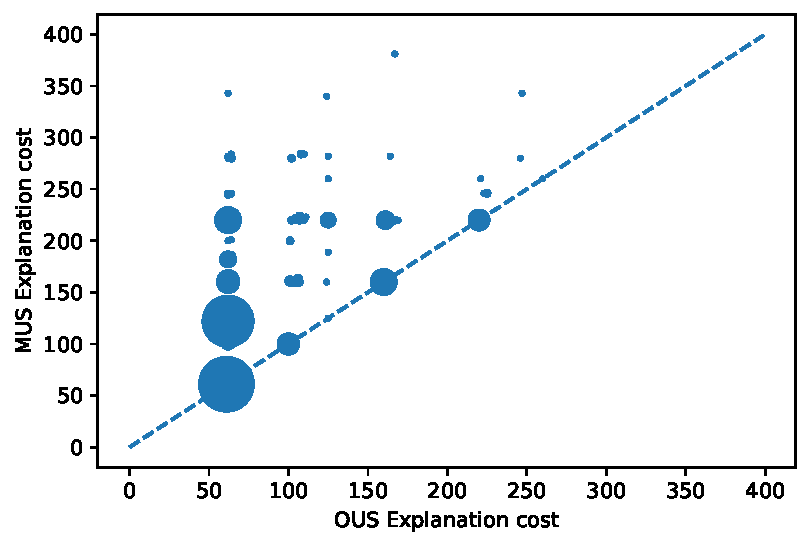
\includegraphics[width=\columnwidth]{figures/rq1.pdf}
  \caption{Q1 - Optimal vs Greedy explanation generation quality}
  \label{fig:rq1}
\end{figure}


\paragraph{Explanation quality} 
Similar to \citet{ecai/BogaertsGCG20}, a weight assigned to each type of constraint used. The weighted sum of the constraints present in the 
(\textit{minimum} / \textit{optimal}) 
% minimal/optimal
unsatisfiable subset become a proxy to how difficult the generated explanation really is.
% commaring the explanation quality of mus and ous
To answer \textbf{Q1}, we start by generating a sequence of explanations using the \comus from an initial assignment $I_0$.. Then, using this sequence as a starting point, we look for a MUS-based explanation given the partial assignments $I_i$ at step i.
Figure \ref{fig:rq1} depicts how the quality of the MUS-based explanations compare to the OUS approach for all puzzles. Every dott represents a pair of OUS and MUS costs, where the size of the dott relates to the occurence of that pair in the generated sequences.
Note that, the distribution of the dotts show the quality of the OUS explanation is either similar, when along the same-cost diagonal or better in the upper part of the graph. The dotts' sizes demonstrates that the optimal approach will find many easy explanations contrary to the MUS. This confirms the need for \comus approach, which repeatedly looks for the next best explanation given an interpretation.
\begin{table}[ht]
  \centering
  \begin{tabular}{r||c|c|c|c|c}
    % \begin{tabular}{|r||c|c|c|c|c|c|}
      % \hline
      \textbf{p} & \textbf{MUS} & \textbf{OUS}  & \textbf{OUS+I} & \textbf{\comus} & \textbf{\comus+I} \\
      \hline
      1 &       569 &         4114 &     4727 &           803 &         \textbf{299} \\
      2 &       438 &         3834 &     3972 &           607 &         \textbf{238} \\
      3 &       477 &         4220 &     4938 &           932 &         \textbf{607} \\
      4 &       624 &         3508 &     4820 &           388 &          \textbf{97} \\
      5 &      3382 &         Timeout &     Timeout &          3556 &        \textbf{1537} \\
      6 &       568 &         3849 &     3854 &           498 &         \textbf{155} \\
      7 &       372 &         4411 &     4380 &           685 &         \textbf{414} \\
      8 &       474 &         4679 &     5552 &           669 &         \textbf{448} \\
      9 &       766 &         Timeout &     Timeout &          2383 &        \textbf{1135} \\
      p &       224 &         2601 &     2528 &           651 &         \textbf{537} \\
      % \hline
    \end{tabular}
    \caption{Computation time (s) compared between executions}
    \label{table:computationTime}
  \end{table}

To answer \textbf{Q2} and \textbf{Q3}, we depict the total runtime of different configurations in Table \ref{table:computationTime}: p is the puzzle name\footnote{following the naming of the puzzles introduced in \citet{ecai/BogaertsGCG20}}, 
\emilio{MUS : something ?},
\emph{OUS} algorithm \ref{alg:oneStep} from \citet{ecai/BogaertsGCG20} where the MUS call is replaced by the \emph{OUS} solver.
We compare the following enhancements options to the basic \emph{OUS} algorithm: incrementality by reusing satisfiable subsets between \omus calls (+I), constrainedness in the search for explanations (C).


\paragraph{Computation Time} The naïve \omus approach requires significantly more time to find an optimal MUS. This observation demonstrates that the problem complexity increases when a optimality criterion kicks in. We observe that reusing information throughout the calls to the OUS solver burdens the \onestep algorithm with extra processing in order to keep track of all generated satisfiable subsets.


\paragraph{Constrainedness}
Adding constraindness has two major implications.
First, by guiding the search towards the next cheapest optimal explanation using algorithm \ref{alg:oneStepOCUS}, we effectively reduce the amount of calls to the \omus solver.
The constrainedness enhancement as shown in Table \ref{table:computationTime} proves the importance of our approach.
The explanation generation times for a whole sequence are closer and sometimes even better than the MUS approach even though the problem of finding a OUS is more difficult than finding a MUS.

Second, in practice constrainedness is easily combined with incrementality.
The MIP solver is instantiated only once and is reused across the different \onestep calls of algorithm \ref{alg:oneStepOCUS}.
By keeping the MIP solver warm, we take advantage of its efficiency to handle the many satisfiable subsets which are represented under the form of constraints on the variables of the problem specification.
Table \ref{table:computationTime} demonstrates that contrary to to \emph{OUS+I}, incrementality in \textbf{\comus+I} significantly decreases the overall computation time.

\begin{figure}[ht]
  \centering
  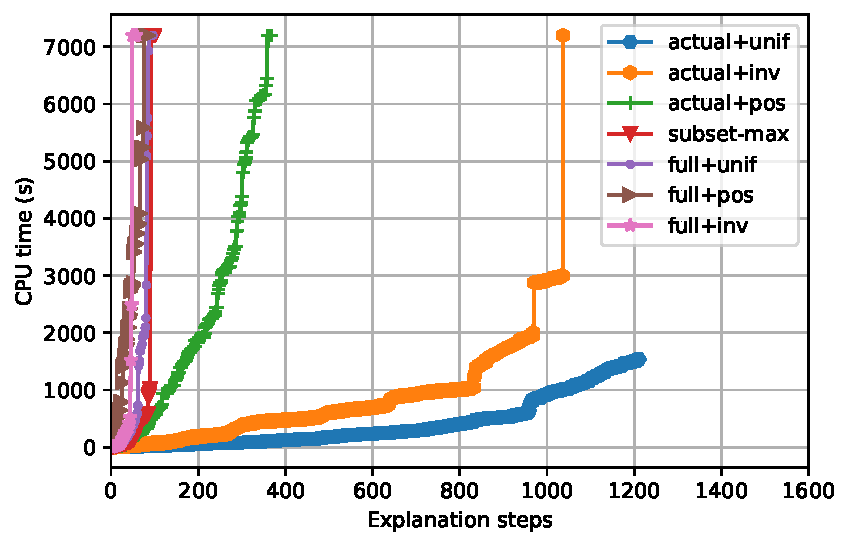
\includegraphics[width=\columnwidth]{figures/rq4.pdf}
  \caption{Q4 - Grow strategies until timeout or full explanation sequence generation}
  \label{fig:rq4}
\end{figure}


\paragraph{Domain-specific \grow} Finally, the core computation of explanations not only lies in the calls to the optimal hitting set solver, but more importantly in computing \emph{high quality} satisfiable subsets.

The latter is reflected in Figure \ref{fig:rq4}.
There are \emilio{some more here!}

% \begin{table*}[]
%     \centering
%     \caption{Execution time generic grow version}
%     \begin{tabular}{|r||c|c|c|c|c|}
%     \hline
%       p &             sat &          subset &      maxsat\_pos &     maxsat\_inv &    maxsat\_unif \\
%     \hline
%      6 &  15.25 - [18]  &  17.46 - [33]  &  48.41 - [9]  &  14.24 - [9]  &  14.71 - [16]  \\
%      8 &  38.95 - [6]  &  21.31 - [10]  &  1558.78 - [6]  &  14.26 - [6]  &  26.47 - [6]  \\
%      p &  14.09 - [9]  &  19.96 - [10]  &  646.94 - [9]  &  6.66 - [1]  &  9.84 - [4]  \\
%      2 &  18.6 - [9]  &  10.12 - [15]  &  171.94 - [9]  &  14.62 - [7]  &  16.54 - [7]  \\
%      7 &  10.24 - [7]  &  17.52 - [8]  &  1542.48 - [1]  &  13.03 - [1]  &  12.31 - [4]  \\
%      1 &  26.25 - [13]  &  20.52 - [13]  &  333.4 - [13]  &  13.28 - [12]  &  16.49 - [13]  \\
%      4 &  40.52 - [101]  &  22.86 - [108]  &  360.07 - [16]  &  14.18 - [11]  &  16.59 - [20]  \\
%      10 &  13.75 - [8]  &  26.72 - [8]  &  487.54 - [2]  &  17.88 - [4]  &  13.89 - [4]  \\
%      3 &  22.58 - [21]  &  19.57 - [10]  &  319.77 - [10]  &  13.49 - [9]  &  14.92 - [9]  \\
%     \hline
%     \end{tabular}
% \end{table*}





\ignore{
We now experimentally validate the the performance of the different versions of our algorithms for explaining satisfiable constraint satisfaction problems.

We consider the following benchmarks: CNF instances from the SATLIB problems Benchmark \cite{hoos2000satlib} and a CNF encoding of the logic grid puzzle ``Origin'' of \cite{ecai/BogaertsGCG20}. All code was implemented in Python on top of %CPpy~\footnote{} and
PySAT.\footnote{\url{https://pysathq.github.io}} The MIP solver used is Gurobi 9.0 and when a (Max)SAT solver is used it is RC2 as bundled with PySAT. Experiments were run on a Intel(R) Xeon(R) CPU E3-1225 with 4 cores and 32 Gb memory, running linux 4.15.0.

Based on the theoretical findings of the previous sections, we aim to answer the following research questions:
\begin{compactdesc}
\item[RQ1] what is the effect of postponing optimal hitting set computation, of incremental OUS solving and of pre-seeding \satsets when solving multiple variants of the same problem?
\item[RQ2] how do the different variants of \omus perform when explaining an elaborate constraint satisfaction problem?
\ignore{
\item[RQ3] how do the sequences found when using (constrained) \omus search compare to those found using a heurisic MUS approach?
}
\end{compactdesc}


\paragraph{RQ1}
To answer the first research question, we use 10 CNF instances from the SATLIB Benchmark and randomly choose 10 literals that are entailed by the CNF. For each variant of the algorithm, we compute the OUS of the same 10 literals in the same order within a total time limit of 10 minutes. 
We compare the following enhancements options to the basic \omus algorithm: postponing optimization (+P), incrementality by reusing satisfiable subsets between \omus calls (+I), and pre-seeding $\satsets$ as described in Section~\ref{sec:incremental} (+W). Options can be combined, for example {\omus}+IPW characterises running the \omus algorithm postponing the optimization phase, with incrementality between the successive calls, and warm starting (pre-seeding) with satisfiable subsets of the original CNF formula.
%The executions are set to timeout after 10 minutes, a limit fixed based on the results of experiment 2.

% \rule{\textwidth}{10pt}

% \begin{table*}[t!]
%     \centering
%     \begin{tabular}{|c|c|c|c|c|c|c|c|c|}
%         \hline
%         % p    & nv& nc&           \omus &      {\omus}+Incr &      {\omus}+Post &  {\omus}+Incr+Warm &   {\omus}+Incr+Post & {\omus}+Incr+Post+Warm \\
%         p    & nv& nc&           \omus &      {\omus}+I &      {\omus}+P &  {\omus}+IW &   {\omus}+IP & {\omus}+IPW \\
%         \hline
%         aim-50-1\_6-yes1-4 & 50& 80&   0.88 s  &   0.38 s  &   0.37 s  &   0.81 s  &    0.65 s  &      \textbf{0.33} s  \\
%         par8-2 & 350 & 1157 &   122.42 s  &  94.07 s  &  96.84 s  &  120.55 s  &  126.15 s  &     \textbf{87.31} s  \\
%         zebra\_v155\_c1135 & 155& 1135&   130.38 s  &  87.97 s  &  84.75 s  &  104.7 s  &  124.48 s  &     \textbf{80.92 s}  \\
%         \hline
%         \end{tabular}
%         \caption{Execution time of the \omus variants for deriving 10 literals evaluated on CNF instances.}
%         \label{table:experiment1}
% \end{table*}

% \begin{table*}[t!]
%     \centering
%     \begin{tabular}{|c|c|c|c|c|c|c|c|c|}
%         \hline
%         % p    & nv& nc&           \omus &      {\omus}+Incr &      {\omus}+Post &  {\omus}+Incr+Warm &   {\omus}+Incr+Post & {\omus}+Incr+Post+Warm \\
%         p    & nv& nc&           \omus &      {\omus}+I &      {\omus}+P &  {\omus}+IW &   {\omus}+IP & {\omus}+IPW \\
%         \hline
%         % 1 & 50& 80&   0.88 s  &   0.38 s  &   0.37 s  &   0.81 s  &    0.65 s  &      \textbf{0.33} s  \\
%         % 2 & 350 & 1157 &   122.42 s  &  94.07 s  &  96.84 s  &  120.55 s  &  126.15 s  &     \textbf{87.31} s  \\
%         % 3 & 155& 1135&   130.38 s  &  87.97 s  &  84.75 s  &  104.7 s  &  124.48 s  &     \textbf{80.92 s}  \\
%         par8-5  & 350  & 1171&      --- &     --- &     --- &     --- &      --- &        --- \\
%         par16-1 & 317 & 1264           &      --- &  --- &  --- &     --- &      --- &     --- \\
%         par16-2& 349 & 1392         &      --- &     --- &     --- &     --- &      --- &        --- \\
%         par16-3 & 334 & 1332        &      --- &     --- &     --- &     --- &      --- &        --- \\
%         par16-4-c & 324 & 1292        &      --- &     --- &     --- &     --- &      --- &        --- \\
%         par16-4  & 1015 & 3324        &      --- &     --- &     --- &     --- &      --- &        --- \\
%         hanoi4  & 718 & 4934       &      1 &     1 &     1 &     1 &      1 &        1 \\
%         \hline
%         \end{tabular}
%         \caption{Number of decision variables explained by the variants of the \omus for timed-out CNF instances.}
%         \label{table:experiment1}
% \end{table*}

% \begin{table*}[t!]
%     \centering
%     \begin{tabular}{c|cccc|cccccc}
%         % \hline
%         p &  time [s] &  \#steps &   $\overline{cost}$ & max(cost) &    1 bij &  1trans &  1 clue & 1 clue+i & 1 mult-i & mult-c. \\
%         \hline
%         1 &  1287.27 &     115 &     25.87  &    25.87  &  31.83\% &  50.57\% &  1.09\% &    16.52 \% &     0\% &    0.0\% \\
%         % \hline
%         \end{tabular}
%         \caption{Puzzle Properties, execution statistics and explanation sequence composition for the origin puzzle.}
%         \label{table:experiment3}
% \end{table*}

% ------------------------------- EMILIO LOCK -----------------------------------------
The results can be seen in Table \ref{table:experiment1} and can be summarized as follows: p, nv and nc represent the instance name, the number of variables and the number of clauses respectively. 
Only for instances aim-50-1\_6-yes1-4, par8-2.cnf and zebra\_v155\_c1135.cnf, is the algorithm able to complete the search for OUSs on the 10 decision variables within the required time constraint of 10 minutes.
For these instances, the overall winner is \emph{{\omus}+IPW}. 
All variants time out on the larger instances (par8-5, par16-1, par16-2, par16-3, par16-4-c, par16-4, hanoi4) before finding the OUSs for all 10 decision variables. For instance par8-5, all variants are able to find 6 out of the 10 variables. On all instances that timed-out, \emph{{\omus}+IPW} remains the fastest. Similar results are observed for the remaining instances for all variants par16-* and hanoi4 with the \omus found for only 1 variable.


A further analysis of the overall execution times highlights that much time is spent in the grow procedure, for which we start from the partial assignment found by the SAT check and use the RC2 MaxSAT solver to complete it. 
We reran the same experiments with a greedy grow algorithm instead and observed that \omus is not even able to finish for zebra\_v155\_c1135 and all runtimes increase considerably.
Furthermore, we see that in this case postponing the MIP call effectively redistributes 50\% of the computational load to growing \satsets and the remaining 50 \% are evenly distributed between (i) the SAT solver, (ii) the MIP solver, and (iii) the the greedy and incremental hitting set heuristics. Hence, while the portion of time spent growing satisfiable subsets is reduced, much more iterations are needed to find the optimal OUSs. %runtime of grow is decreased, the number of 
% A further analysis of the overall execution times highlights that the main bottleneck of the algorithm is the time spent WE NEED TEXT HERE AFTER TEH RUNS ARE READY\todo{emilio}

From this experiment we conclude that in the short time limit provided, the best configuration for computing multiple related OUS's is \emph{{\omus}+IPW}, taking advantage of the repeated calls to the OUS algorithm, thus reusing the computed \satsets.
% ------------------------------- EMILIO LOCK -----------------------------------------

% \begin{table*}[h!]
%     \begin{tabular}{|c|c|c|c|c|c|c|c|c|}
%         \hline
%         % p    & nv& nc&           \omus &      {\omus}+Incr &      {\omus}+Post &  {\omus}+Incr+Warm &   {\omus}+Incr+Post & {\omus}+Incr+Post+Warm \\
%         p    & nv& nc&           \omus &      {\omus}+I &      {\omus}+P &  {\omus}+IW &   {\omus}+IP & {\omus}+IPW \\
%         \hline
%         1 & 50& 80&   0.88 s  &   0.38 s  &   0.27 s  &   0.81 s  &    0.65 s  &      0.33 s  \\
%         2 & 350 & 1157 &   22.42 s  &  14.07 s  &  76.84 s  &  20.55 s  &  126.15 s  &     87.31 s  \\
%         3 & 155& 1135&   130.38 s  &  87.97 s  &  64.75 s  &  104.7 s  &  124.48 s  &     80.92 s  \\
%         4..10 & x $\cdot$ $10^2$ & x $\cdot$ $10^3$           &      --- &     --- &   --- &  --- &   --- &     --- \\
%         % 5 & 317 & 1264           &      --- &  --- &  --- &     --- &      --- &     --- \\
%         % 6 & 324 & 1292        &      --- &     --- &     --- &     --- &      --- &        --- \\
%         % 7 & 334 & 1332        &      --- &     --- &     --- &     --- &      --- &        --- \\
%         % 8& 349 & 1392         &      --- &     --- &     --- &     --- &      --- &        --- \\
%         % 9  & 1015 & 3324        &      --- &     --- &     --- &     --- &      --- &        --- \\
%         % 10  & 718 & 4934       &      --- &     --- &     --- &     --- &      --- &        --- \\
%         \hline
%         \end{tabular}
%         \caption{Comparison of \omus variants evaluated on CNF instances.}
%         \label{table:experiment1}
% \end{table*}

% \begin{table*}
%     \begin{tabular}{|c|c|c|c|c|c|c|}
%         \hline
%         p                  &           \omus &      {\omus}+Incr &      {\omus}+Post &  {\omus}+Incr+Warm &   {\omus}+Incr+Post & {\omus}+Incr+Post+Warm \\
%         \hline
%         1 &    0.88 s | 10 &   0.38 s | 10 &   0.27 s | 10 &   0.81 s | 10 &    0.65 s | 10 &      0.33 s | 10 \\
%         2            &   22.42 s | 10 &  14.07 s | 10 &  76.84 s | 10 &  20.55 s | 10 &  126.15 s | 10 &     87.31 s | 10 \\
%         3  &  130.38 s | 10 &  87.97 s | 10 &  64.75 s | 10 &  154.7 s | 10 &  124.48 s | 10 &     80.92 s | 10 \\
%         4            &      600 s | 1 &  600 s | 2 &  600 s | 1 &     600 s | 1 &      600 s | 1 &     600 s | 1 \\
%         5         &      600 s | 1 &     600 s | 1 &     600 s | 1 &     600 s | 1 &      600 s | 1 &        600 s | 1 \\
%         6         &      600 s | 1 &     600 s | 1 &     600 s | 1 &     600 s | 1 &      600 s | 1 &        600 s | 1 \\
%         7         &      600 s | 1 &     600 s | 1 &     600 s | 1 &     600 s | 1 &      600 s | 1 &        600 s | 1 \\
%         8          &      600 s | 6 &     600 s | 6 &     600 s | 2 &     600 s | 6 &      600 s | 2 &        600 s | 2 \\
%         9         &      600 s | 1 &     600 s | 1 &     600 s | 1 &     600 s | 1 &      600 s | 1 &        600 s | 1 \\
%         10            &      600 s | 6 &     600 s | 6 &   600 s | 6 &  600 s | 6 &   600 s | 6 &     600 s | 6 \\
%         \hline
%         \end{tabular}
%         \caption{Comparison of \omus variants evaluated on CNF instances.}
%         \label{table:experiment1}
% \end{table*}


\paragraph{RQ2}
The second research question is: how do the different variants perform when explaining an elaborate constraint satisfaction problem? For this, we tested the complete generation of an explanation sequence. 
In this comparison, we expect that constrained versions of our algorithm perform best as they will allow performing an entire step of the explanations in a single call.
For this reason, we only include different variations on the constrained configuration and the single best variant of non-constrained algorithms found in the previous experiment. 

% \begin{figure}[t]
%     \centering
%     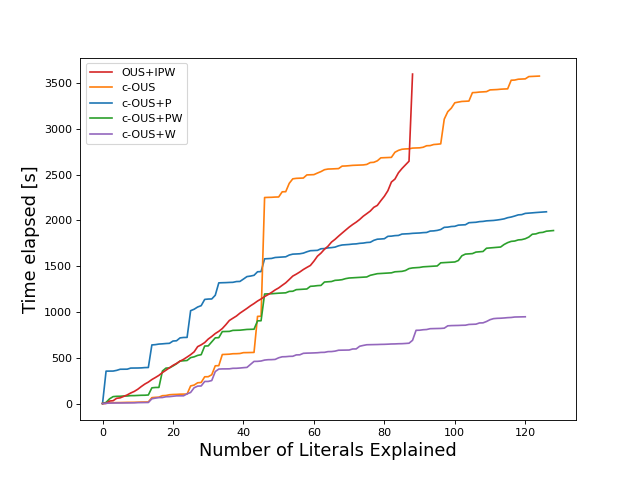
\includegraphics[width=\columnwidth]{figures/omusConstrCumulative.png}
%     \caption{Experiment 2}
%     \label{fig:exp2}
% \end{figure}

We generate the explanation sequence as far as possible within a time limit of one hour. 
The results for the  ``origin'' puzzle is shown in Figure~\ref{fig:exp2}.
It shows the number of literals explained on the X-axis, and the cumulative time taken on the Y-axis. 
Only three configurations find the full explanation sequence (note that there can be multiple optimal sequences with a different length, which explains the difference in length between the configurations).
We  see that the best non-constrained implementation is unable to explain all of the literals within the time limit; especially around step 95 there is a big jump in runtime. The vanilla constrained-OUS approach is not able to finish in time either, with big jumps in time on specific (large and costly) explanation steps.

When combining constrained-OUS with either pre-seeding, post-poned optimisation or both, then our approach is able to fully explain the solution. Best results are obtained with constrained-OUS with just pre-seeding at the beginning. The post-poned optimisation in this case may spent a lot of time generating MCSs that are not or little relevant to the constrained OUSs we are seeking. 

\paragraph{Concluding notes}
While a direct comparison of the runtime needed to find an explanation sequence of our tool versus the one of \citet{ecai/BogaertsGCG20} %built on the IDP system \cite{WarrenBook/DeCatBBD14} 
would shed more light on the performance impact, we can not do a fair comparison as the solvers and hardware used are different.

However, the authors reported that explaining a single puzzle easily takes one to two hours due to the many MUS calls. In contrast, Figure~\ref{fig:exp2} shows that three of our constrained-OMUS approaches fully explain a puzzle one of their larger puzzles in 20 to 30 minutes.
Furthermore, our algorithms guarantee that each explanation step is \emph{optimal} with respect to $f$. As such we know that the generated sequences are at least as good for the cost function provided.

% do not include such an extensive experiment here since it would not be a fair comparison of the underlying algorithms. Indeed, different solving technology is used for finding MUSs, and satisfying assignments. 
%We can, however, give an indication of the speed by mentioning that in some preliminary experiments (e.g., on the origin puzzle), using constrained \omus calls, we can find the entire sequence in roughly 20 minutes, whereas the IDP-based tool takes over two hours.


% Finally, for \textbf{RQ3} \emilio{Bart: concluding phrases on expl. generation}
%  we compare the sequence found by our proposed method with the sequence reported on in~\cite{ecai/BogaertsGCG20} for the origin puzzle (puzzle 1). 
% The explanation sequence for the puzzle is generated using \omus Constr with pre-seeding and according to the same cost function as Bogaerts et al.~\cite{ecai/BogaertsGCG20}. We report statistics relating to the explanation generation in table~\ref{table:experiment3}.
% Evidently, one of the most important observations is the speed-up provided by \omus Constr. 
% As a matter of fact, the sequence is generated in a bit more than 21 minutes compared to a few (2-3) hours in~\cite{ecai/BogaertsGCG20}, meaning that \omus Constr is 8-10x faster, while also finding the optimal explanations in each step.
% Table \ref{table:experiment3} also reports that the explanation sequence has become easier to understand: the average cost is slightly lower and so is $max(cost)$, the cost of the most difficult explanation in the puzzle. 


% \begin{table*}
%     \begin{tabular}{ccc|ccc|cccccc}
%         % \hline
%         types &  $|dom|$ &  $|grid|$ &  time [s] &  \#steps &    cost &    1 bij &  1trans &  1 clue & 1 clue+i & 1 mult-i & mult-c. \\
%         \hline
%         4 &      5 &     150 &  1287.27 &     115 &        25.87 &  27.83\% &  49.57\% &  6.09\% &    11.3\% &     5.22\% &    0.0\% \\
%         % \hline
%         \end{tabular}
%         \caption{Puzzle Properties, execution statistics and explanation sequence composition for the origin puzzle.}
%         \label{table:experiment3}
% \end{table*}

%
%\begin{figure*}[ht]
%    \centering
%    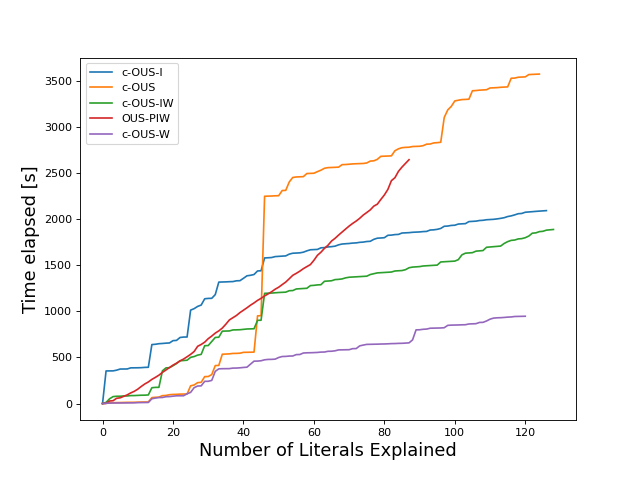
\includegraphics[width=\columnwidth]{figures/omusNonConstrCumulative.png}
%    \caption{}
%    \label{}
%\end{figure*}

% \begin{figure}[ht]
%     \centering
%     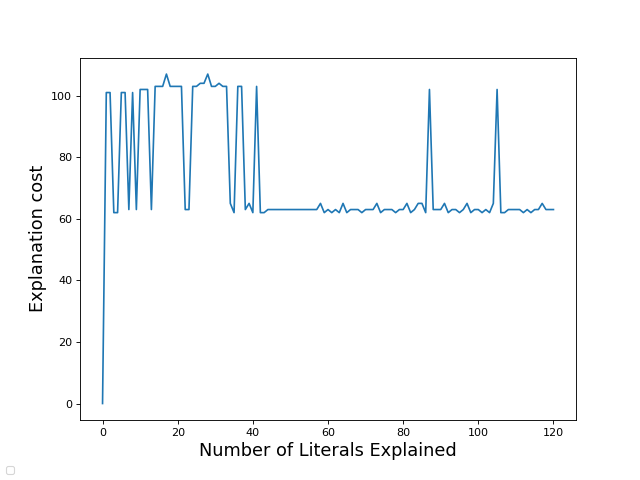
\includegraphics[width=\columnwidth]{figures/explanation_cost.png}
%     \caption{}
%     \label{}
% \end{figure}

}

% \section{Discussion}   
% \todo{1 1/2 column} 
% \begin{itemize}
    \item yes
\end{itemize} 

\section{Related Work}\label{sec:related}
% \todo{1 column}
% {\color{OliveGreen} OLD TEXT TO BE REWRITTEN
% !TeX root = ./main.tex

\begin{itemize}
    \item XAIP
    \item Smallest MUS (QMaxSAT, Ignatiev)
    \item MaxHS-nonOPT
\end{itemize}
% }


\section{Conclusion, Challenges and Future work}\label{sec:conclusion}
% \todo{1/2 column}
% !TeX root = ./main.tex
We presented a \hitsetbased algorithm for finding \textit{optimal constrained} unsatisfiable subsets, with an application in generating explanation sequence for constraint satisfaction problems. Constrainedness, incrementality and a domain-specific \grow method were key to generating such sequences in a reasonable amount of time.

%Summarised, while \citet{ecai/BogaertsGCG20} had to generate many MUSs for finding a single next explanation step, the step-wise explanation generation directly benefits from the \comus approach of finding the optimal explanation candidate at any point in the sequence.

%There are many trade-offs to be made in the algorithm, including time spent computing optimal or non-optimal hitting sets, how to reuse information and how to grow the satisfiable subsets. While we studied the key algorithmic dimensions of information reuse, a deeper study of alternative approaches to balance these trade-offs is needed, for instance comparing different methods to grow a satisfiable subset, and balancing the trade-off between finding hitting sets of high quality versus having to compute fewer hitting sets.


With the observed impact of different `\grow' methods, an open question remains whether we can quantify precisely and in a generic way what a \textit{good} or even the best set-to-hit is in a hitting set approach. 
While we focused on generating entire sequences, another question could be what the best method is for finding a single explanation step, that is a single OCUS. 
This would be important for example in interactive configuration applications~\cite{van2017kb}; where incrementality can also play across different queries.
The synergies of our approach with the more general problem of QMaxSAT \cite{DBLP:journals/constraints/IgnatievJM16} is another open question.

%The goal of explaining satisfaction problems fits in wider goal of human-machine decision making, which is related to interactive constraint solving~\cite{putnam2019toward}. The use of MUSs in this context has been explored by . For interactivity, finding a single O(C)US fast would be the focus, where incrementality can play a big role.

The concept of OUS, incremental OUS and constrained OUS are not limited to explanations of satisfaction problems and we are keen to explore other applications too.
A general direction here are \textit{optimisation} problems and the role of the objective function in explanations.
%From the explanation point of view, a next challenge is how to compute explanations for optimisation problems, that is, where decisions are made based on search and not just propagation. We believe a constrained OUS algorithm can also play a key part in that. Finally, an open challenge is that of defining appropriate cost functions for generating explanations, including how to evaluate what a ``good'' explanation sequence is. While we currently find a sequence where each step is optimal with respect to the cost function, we have yet to consider whether it is possible to optimize a cost function over the entire sequence as well.
Within satisfaction, both MUSs and \hitsetbased algorithms are also investigated in the context of explaining machine learning decisions~\cite{ignatiev2019abduction}. 
In this context, an open direction for future work is to examine the potential benefit of using optimal MUS search and whether constrainedness properties can further boost its possibilities.
%\begin{itemize}
%    \item Conclusion on resutls
%    \item Challenges next : extension to XOPT ? 
%    \item Applicability on other problems ?
%    \item Characterizing explanation difficulty
%\end{itemize}

\paragraph{Acknowledgments}
\textit{This research received partial funding from the Flemish Government (AI Research Program) and the FWO Flanders project G070521.}

\ignore{
\newpage
{\color{red}This should be page (at most) 7. Limit is 6 real pages, 1 page of references. Proofs go in appendix. If references are too long, I will shorten them. That is not an issue}
\newpage
}

{
    % \fontsize{8}{6}
%% The file named.bst is a bibliography style file for BibTeX 0.99c
\bibliographystyle{named}
\bibliography{krrlib,mybibfile,ref} 
}
% \bibliographystyle{ijcai21}


\end{document}

I REMOVED ALL OF THE REST SINCE IT MESSES UP OUR NUMBERINGS
% !TeX root = ./main.tex
\clearpage
\begin{algorithm}[ht]
    \Input{${\cal C}$,  \textit{a CNF ${\cal C}$ over a vocabulary $V$} }
    \Input{$U$, \textit{a user vocabulary $U \subseteq V$} }
    \Input{$f$, \textit{a cost function $f : 2^{lits({U})} \rightarrow  \mathbb{N} $.}}
    \Input{$I$, \textit{a partial interpretation over $U$}}
    \Output{$E$, \textit{a sequence of explanation steps as implications $I_{expl} \implies N_{expl}$}}
    % \vspace*{0.01cm}
    % \DontPrintSemicolon
    \caption{$\call{ExplainCSP}(\formulac, U, f, I)$}
    \label{alg:explainCSP2}
    $\sat \gets \initsat({\cal C}$) \;
        % \tcp{Hyp: f}
    $E \gets \langle \rangle$\;
    $I_{end} \gets \optprop(U, I)$ \;
    %$U \gets U \cap I_{end}$ \;
    %$I_{expl} = \{i \in I_{end} | f(i) < inf \wedge f(-i) < inf\}$ \;
    % \algemilio{bart: What's a better way to get the initial interpr.?}
    % $I \gets \{l \in I_{end} | f(\lnot l) = inf\}$ \;
    \While{$I \neq I_{end}$}{
        %$E \gets \call{bestStep}({\cal C},U, f,\Iend, I)$\;
        $X \gets \call{bestStep}({\cal C},f,\Iend, I)$\;
        $I_{\mathit{best}} \gets I \cap X$\;
        %$\formulac_{\mathit{best}}\gets \formulac\cap X$\;
        $N_{\mathit{best}} \gets \optprop(U, I_{\mathit{best}}) \setminus I$\;
        %add $\{I_{\mathit{best}} \wedge \formulac_{\mathit{best}} \implies N_{\mathit{best}}\}$ to $E$\;
        add $\{I_{\mathit{best}} \implies N_{\mathit{best}}\}$ to $E$\;
        $I \gets I \cup N_{\mathit{best}}$\;
    }
    \Return{E}\;
\end{algorithm}

\begin{algorithm}[ht]
    \DontPrintSemicolon
    \Input{$U$, \textit{a user vocabulary $U \subseteq V$} }
    \OptInput{$I$, \textit{a partial interpretation over $U$.} }
    \State{$\sat$, \textit{a $\sat$ solver initialised with a CNF.}}
    \Output{\textit{The projection onto U of the intersection more precise than $I$.}}
    \label{alg:optprop}
    $sat?,\mu \gets \sat.\texttt{solve(}I\texttt{)}$\;
    $\mu \gets \{l \mid \texttt{var}(l) \in U \}$\;
    $b \gets$ a new blocking variable\;
    % \algemilio{Should I add the blocking variables $b_i$ to the newly added clause ?}
    \While{true}{
        % \sout{${\cal C} \gets {\cal C} \wedge (\lnot b_i \underset{l \in \mu}{\bigvee} \lnot l)$}\; 
        $\sat.\texttt{addClause(}\lnot b_i \underset{l \in \mu}{\bigvee} \lnot l\texttt{)}$\;
        % add $(\lnot b_i \underset{l \in \mu}{\bigvee} \lnot l)$ to $\sat$ solver\; 
        $sat?,\mu' \gets \sat.\texttt{solve(}I \wedge \{b_i\}\texttt{)}$\;
        \If{ $not$ $ sat?$}{
            $\sat.\texttt{addClause(}\lnot b_i\texttt{)}$\;
            \Return{$\mu$} \;
        }
        $\mu \gets \mu \cap \mu' $\;
    }
    \caption{$\call{OptimalPropagate}(\uservars [, I], \sat)$}
\end{algorithm}


\begin{algorithm}[ht]
    \DontPrintSemicolon
    \caption{$\call{bestStep--c-OUS}(f,\Iend, I, \sat)$}
    \label{alg:singleStepExplain3}
    % \Input{${\cal C}$, \textit{a CNF}.}
    \Input{$f$, \textit{a cost function $f : 2^{{\cal G}} \rightarrow  \mathbb{N} $ over CNF ${\cal G}$}.}
    \Input{$I_{end}$, \textit{the cautious consequence, the set of literals that hold in all models}.}
    \Input{$I$, \textit{a partial interpretation s.t. $I \subseteq I_{end}$}.}
    \State{$\sat$, \textit{a $\sat$ solver initialised with a CNF.}}
    \Output{\textit{a single best explanation step}}
    \vspace*{0.01cm}
    ${\cal A} \gets I \cup (\overline{\Iend} \setminus \bar{I})$ \tcp*{Optimal US is subset of A}
    set $p \triangleq \underset{l \in \overline{\Iend}}{\sum} l = 1$  i.e. exactly one of $\overline{\Iend}$ in the unsatisfiable subset. \; %\textit{and} none of $\{I_{end} \setminus I\}$ \textit{and} none of $\bar{I}$ can be in the hitting set\;
    % \Return{$\comus(f,p, {\cal A})$}\;
\end{algorithm}


\begin{algorithm}[ht]
    % \Input{${\cal C}$, \textit{a CNF}.}
    \Input{$f$, \textit{a cost function $f : 2^{{\cal A}} \rightarrow  \mathbb{N} $.}.}
    \Input{$p$, \textit{a predicate $p: 2^{{\cal A}} \rightarrow \{ t, f\}$.}.}
    \Input{$A$, \textit{a set of assumption literals, s.t. ${\cal C} \cup A$ is unsatisfiable.}}
    \State{$\sat$, \textit{a $\sat$ solver initialised with a CNF.}}
    % \Output{\textit{$(p, f)-OUS$, a subset ${\cal A}'$ of ${\cal A}$ that satisfies $p$ s.t. ${\cal C} \cup {\cal A}'$ is $UNSAT$ and  ${\cal A}'$ is $f$-optimal.}}
    \Output{\textit{$(p, f)-OUS$, a subset ${\cal HS}$ of ${\cal A}$ that satisfies $p$ s.t. ${\cal C} \cup {\cal HS}$ is $UNSAT$ and  ${\cal HS}$ is $f$-optimal.}}
    % \tcp{Hyp: ${\cal C} \cup A$ is unsatisfiable}
    \DontPrintSemicolon
    $\setstohit \gets \emptyset$ \;
    % $mode \gets $ \texttt{OPT} \;
    \While{true}{
        % ${\cal A}' \gets \cohs(f, p, {\cal A}, \setstohit) $  \;%\tcp*{\small Find \textb    $\setstohit  \gets \setstohit  \cup \{  \formula \setminus \F''\}$ \;
    %     % ${\cal A}' \gets \chs(f, p, {\cal A}, \setstohit) $  \;%\tcp*{\small Find \textb    $\setstohit  \gets \setstohit  \cup \{  \formula \setminus \F''\}$ \;
        ${\cal HS} \gets \cohs(f, p, {\cal A}, \setstohit) $  \;%\tcp*{\small Find \textb    $\setstohit  \gets \setstohit  \cup \{  \formula \setminus \F''\}$ \;
    %     % \emilio{
        \tcp{Add mode to algorithm for postponing optimisation. Mode switch corresponds to switching between heuristic conditional Hitting set computation and the optimizer.}\;
        $sat?,\ \mu \gets \sat({\cal HS})$\;
    %     % $sat?,\ {\cal A}'' \gets \sat({\cal HS}')$\;
    %     % $sat?,\ {\cal A}'' \gets \sat({\cal A}' \mid \{ {\cal A}'' \cap I_0\}, A)$\;
        \If{ $\lnot \sat({\cal HS})$}{
            \Return{${\cal HS}$} \;
        }
        % \sout{$A'' \gets  \grow(C, f, p, A',A) $}\;
        % \sout{$\setstohit  \gets \setstohit  \cup \{  A \setminus A''\}$}\; %\tcp*{We can reuse the H across diff call to alg \ref{alg:explainCSP} was $H \cup \{F \setminus F''\}$ }
        $SS \gets  \grow(C, f, p, A, HS) $\;
        $\setstohit  \gets \setstohit  \cup \{  {\cal A} \setminus {\cal SS}\}$\;
    % }
    }
    \caption{$\comus(f,p, {\cal A}, \sat)$}
    % \label{alg:comus}
\end{algorithm}

\color{red}
% \ignore{
% TO BE PUT BACK:
\section{Optimal Unsatisfiable Subsets}\label{sec:omus}
\todo{OLD SECTION}OLD SECTION
% \todo{2 column}\label{
% !TeX root = ./main.tex

Before presenting an algorithm that computes optimal MUSs, we first formally define the problem we are going to solve and we present an extension of the hitting set duality of \cref{prop:MCS-MUS-hittingset}. 
Throughout this section, we assume that an objective function $f: 2^\formula \to \nat$ that assigns to each subset of \formula a cost that is fixed. Our goal now is not to find arbitrary MUSs, but unsatisfiable subsets that are optimal with respect to $f$. 


% \begin{itemize}
%   \item Davies'MaxSAT version ? (takes a lot of space on paper)
%   \item OUS v1
%   \item OUS v2
% \end{itemize}
% \emilio{
%   In this section, we first introduce the notion of OUS and extend the smallest MUS approach \cite{ignatiev2015smallest} to compute optimal MUS with respect to an objective function. 
% }
% We further improve the efficiency of the OUS algorithm using ideas from the improved \textsc{MaxHS} algorithm \cite{davies2013postponing}.

\begin{definition}
  A MUS $M$ of \formula, such that no MUS $M'$ exists with $f(M')<f(M)$, is called an \emph{$f$-Optimal Unsatisfiable Subset} (f-OUS) of \formula.
\end{definition}

\begin{definition}
  Let $\m{H}$ be a collection of subsets of a set $S$ and $c$ a function $2^S\to\nat$. 
  A hitting set of $\m{H}$ is called \emph{$c$-optimal} if there are no hitting sets $h'$ of $\m{H}$ with $c(h')<c(h)$. 
\end{definition}
In case our collection of sets $\m{H}$ happen to be subsets of \formula, we can use the function $f$ to measure the costs. 
% 
% While any objective function is applicable for OUSes, the set of possible objective functions is constrained to \emph{monotonic} functions to guarantee that the algorithm \ref{alg:omus} presented below finds the OUS.

% \begin{definition}
%   Given a CNF Formula \formula, let $f : 2^{\formula} \rightarrow \mathbb{R}$ be a mapping of a sets of clauses to real numbers. f is said to be a \emph{monotonic} objective function if for any subsets $\m{A}$, $\m{B}$ of \formula if $\m{A} \subseteq \m{B}$ then $f(\m{A}) \leq f(\m{B})$.
% \end{definition}

The hitting set duality now straightforwardly generalizes as follows. 

\begin{proposition}\label{prop:optimal-hitting-set}
  A set $\m{U} \subseteq \formula$ is an $f$-OUS of \formula iff $\m{U}$ is an $f$-optimal hitting set of \mcses{\formula}.
\end{proposition}
\tias{and inversely? now it is not a duality... perhaps 'the duality allows us to derive the following:'} \bart{The inverse also holds. We can add it (might indeed make more sense), though we only use one direction)}

In order to find an OUS, there is no need to explicitly enumerate all MCSes of \formula. In practice it suffices to compute sufficiently many of them. \tias{missing argument of why being optimal and unsat is sufficient to be the f-ous... because the hs is also a (superset) of a smaller H, an OUS always has to be unsatisfiable, and so any HS of H subset MCS is either SAT or the OUS?}\bart{I added a proof}
% and the correction subsets considered need not neccesarily be maximal. 
The following proposition formalizes this. 
% 
% Lemma \ref{lemma:K} specifies that, in practice, it is not required to enumerate all MCSes of \formula.
% The algorithm only requires finding an optimal hitting set on \mcses{\formula} tat is unsatisfiable.

\begin{proposition}\label{prop:K}
  Let $\m{H}$ be a set of correction subsets of \formula \tias{should be subset of correction subsets $H \subseteq mcss$?} \bart{the way it is phrased now also allows for non-minimal correction sets. Which is needed if grow is nonoptimal}. 
  If $\m{U}$ is an $f$-optimal hitting set of \m{H} and $\m{U}$ is unsatisfiable, then $\m{U}$ is an $f$-OUS of \formula. 
\end{proposition}
\begin{proof}
%   We know that . 
  All that is left to show is $f$-optimality of $\m{U}$.
  If some other unsatisfiable subset $\m{U}'$ exists with $f(\m{U}')\leq f(\m{U})$, we know that $\mu{U}'$ would hit every minimal correction set of \m{F}, and hence also every set in \m{H} (since every correction is the superset of a minimal correction set).
  Since $\m{U}$ is an $f$-optimal hitting and $\m{U}'$ also hits $\m{H}$, it must thus be that $f(\m{U})=f(\m{U'})$. 
%   
\end{proof}


% \begin{proposition}
%   If $\m{U}$ is an $f$-OUS of \formula and $\m{C}$ a correction subset of \formula, then 
% \end{proposition}


We are now ready to present our basic OUS algorithm in \cref{alg:omus}. 
The algorithm keeps track of a set $\m{H}$ of (minimal) correction subsets of $\formula$. 
It makes use of a procedure \ohs that computes an optimal (with respect to $f$) hitting set $\formula'$  of a given set of subsets of \formula.
We take inspiration for the hitting set approach to solving partial weighted MaxSAT~\cite{davies2011solving} and will use a MIP solver to compute the optimal hitting set.
Whenever such a hitting set is found, a \sat-call checks whether the result is satisfiable. If it is, \cref{prop:K} guarantees that the result is an OUS. 
If it is not, we know that the hitting set is a satisfiable subset. We now need to compute and add an MCS which is not hit by the found hitting set.
As is common, we first use a procedure \grow to extend the hitting set to a set $\formula''$ with $\formula'\subseteq \formula''\subseteq\formula$ such that $\formula''$ is still satisfiable. By definition $\formula \setminus \formula''$ is a correction subset; we add this complement to $\m{H}$ \bart{better sentence}. \tias{smth about MSS/MCS, although the way we explain it it needs not be 'maximal', should we also be explicit about that? I don't like the current version.} \bart{For our algorithms, it is crucial that they don't have to be maximal. Otherwise all approximations such as greedy grows would be incorrect}

The implementation of \grow can be achieved in different ways.
In fact, we could call a weighted partial \textsc{MaxSAT} solver to find the maximal satisfiable subset of clauses grown from the hitting set.
In practice, we use a greedy approximative method to find a sastisfying assignment favoring literals that will satisfy the most clauses of highest weights.
More precisely, we rank the clauses based on the ratio of weight to the number of literals not yet assigned in the clause.
\tias{we doen weighted partial maxsat, waarbij we de satisfying solution van de SAT call gebruiken. Details hiervan leiden af van de paper imho, en we hebben geen tijd om te experimenteren wat best is. Mss gewoon:}
... In practice, we use the model found by the SAT call on line 4 and let a maxsat solver extend it to maximally cover $\formula$. We note that typically most literals are part of the found model of $\formula'$ and so this maxsat problem is considerably smaller than $\formula$.
\bart{Akkoord. Na de paper deadline wil ik wel eens weten welke weights we gebruiken...}

\todo{beter uitleggen. Nog niet zo duidelijk. Ook niet zeker of dit op deze moment echt van belang is.}
\bart{OOK: hoe gebruiken we de maxsat solver, zoeken we een MSS met een zo HOOG mogelijke kost? Is dat ``optimaal'' in zekere zin? Ik weet het eigenlijk niet... Een MSS met hoge kost, betekent dat de MCS een lage kost heeft. Maar een MCS met een hoge kost is eigenlijk informatiever, neen? Dat geeft een strengere constraint op onze hitting sets? 
Wel... We willen zo weinig mogelijk constraints in de MCS (om een sterke cosntratint op de hitting set te krijgen), maar we hebben voor die zaken wel liefst GROTE gewichten in de MCS. 
Dus... eerlijk... ik weet niet zo goed of we gewichten hier wel in rekening moeten brengen... En tenzij we het zelf volledig snappen zou ik het niet in de paper schrijven :-)}


% 
% This can be implemented in various ways, e.g., using a MAXsat call can guarantee that $\formula''$ is an MSS of \formula. Another possibility is  -- given a model $I$ of $\formula''$ -- to take $\formula''$ to be $\{c\in\formula \mid I\models c\}$.

% \newcommand\setstohit{\ensuremath{\m{H} }\xspace}
\begin{algorithm}[ht]
  \DontPrintSemicolon
  $\setstohit  \gets \emptyset$ \; %\label{omus-line1} 
  \While{true}{
    $\F' \gets \ohs(\setstohit,f) $ \label{smus-hs} \;%\tcp*{\small Find \textb    $\setstohit  \gets \setstohit  \cup \{  \formula \setminus \F''\}$ \;
% f{optimal} solution}
    % \tcp{\small set with all unique clauses from hitting set}
%     (sat?, $\kappa$) $\gets$ \texttt{SatSolver}($hs$)\;
    % \tcp{If SAT, $\kappa$ contains the satisfying truth assignment}
    % \tcp{IF UNSAT, $hs$ is the OUS }
    \If{ $\lnot \sat(\F')$}{
      \Return{$\F'$} \;
    }
    $\F'' \gets  \grow(\F',\F) $\;
    $\setstohit  \gets \setstohit  \cup \{  \formula \setminus \F''\}$ \;
  }
  \caption{$\omus(\formula,f)$ }
  \label{alg:omus}
\end{algorithm}
\tias{I would add the 'delayed' extension here...}
\bart{Depends on what our core contribution is. I like moving contributions as much to the front of the paper as possible.... }

% 
% \begin{algorithm}[ht]
%   \DontPrintSemicolon
%   $\m{K} \gets \emptyset$  \label{omus-line1} \;
%   \While{true}{
%     $hs \gets$ \texttt{FindMinCostHittingSet}($\m{K}, f$) \label{omus-hs} \;%\tcp*{\small Find \textbf{optimal} solution}
%     % \tcp{\small set with all unique clauses from hitting set}
%     (sat?, $\kappa$) $\gets$ \texttt{SatSolver}($hs$)\;
%     % \tcp{If SAT, $\kappa$ contains the satisfying truth assignment}
%     % \tcp{IF UNSAT, $hs$ is the OUS }
%     \If{ not sat?}{
%       \Return{$(hs,  \m{K})$} \;
%     }
%     $MSS \gets  \texttt{Grow}($hs$) $\;
%     $\m{K} \gets \m{K} \cup \{  \formula$ $\setminus MSS\}$ \;
%   }
%   \caption{\textsc{OUS($\formula, \ f$)}}
%   \label{alg:omus}
% \end{algorithm}


% The \texttt{OUS} algorithm repeatedly computes the optimal hitting set $hs$ (line \ref{omus-hs}) on the already found $\m{K}$, the MCSes of \formula. If the $hs$ is satisfiable, $hs$ is grown grown to 
% The algorithm terminates and $hs$ is guaranteed to be the OUS based on lemma \ref{lemma:K}. 

% From proposition \ref{prop:MCS-MUS-hittingset}, if $hs$ is unsatisfiable, that means it hits all \mcses{\formula}. 
% Furthermore, $hs$ is also a cost optimal hitting set on $\m{K}$. It means that if we add any MCS to $\m{K}$, the cost of other hitting sets will either increase in cost or remain the same.

% Lemma \ref{lemma:K} also 

% Note if we assign a weight to all clauses equal to the number of literals it contains, then we reduce the problem of finding an optimal hitting set back to finding the minimum hitting set.
% % The algorithm then computes the smallest MUS instead of the OUS \cite{ignatiev2015smallest}.
% 
% % \subsection*{Implementation}
% 
% Inspired by the approach of Davies and Bacchus \cite{davies2011solving}, the optimal hitting set problem is formulated as a Linear integer Program and encoded into the MIP solver. 
% Contrary to the \texttt{SMUS} algorithm, which uses the \textsc{SAT} solver to compute minimum hitting sets. 

% The implementation of the grow procedure can be achieved in different ways.
% In fact, we could call a weighted partial \textsc{MaxSAT} solver to find the maximal satisfiable subset of clauses grown from the hitting set.
% In practice, we use a greedy approximation strategy to find a sastisfying assignment favoring literals that will satisfy the most clauses of highest weights.
% More precisely, we rank the clauses based on the ratio of weight to the number of literals not yet assigned in the clause.
% 



% \begin{algorithm*}
%   \DontPrintSemicolon
%   \SetKwSwitch{Switchy}{Case}{Default}{swtich}{}{case}{otherwhise}{}%
%   \Begin{
%     \tcp{F = unsatisfiable CNF formula; M = Collection of MSSes; $f_{cost}$ = cost function}

%     $\m{K} \gets $ $\emptyset$ \;
%     \tcp{grow mss from input mss}
%     \ForEach(){$\m{MSS} \in \m{M}$}{
%       $\m{MSS}' \gets$ {Grow($\formula \cap \m{MSS}$)} \;
%       % $\m{MSS} \gets $  \;
%       $\m{K} \gets \m{K} \cup \{  \formula \setminus \m{MSS}'\}$ \;
%     }

%     % $\m{M} \gets \emptyset$ \;
%     mode $\gets$ mode\_greedy \;
%     % \sout{$\m{H} \gets \m{H}_0$} \;
%     \While{true}{
%       % \tcp{Find a series of non-optimal solutions}
%       \While{true \label{alg:omus-nonOPT-nested-start}}{
%         \Switch{$nonOptLevel$}{
%           \Case{mode\_incr}{
%             $hs \gets$ {FindIncrementalHittingSet}($\m{K}$, $\m{C}$, $hs$)\;
%           }
%           \Case{mode\_greedy}{
%             $hs \gets$ {FindGreedyHittingSet}($\m{K}$)\;
%           }
%         }

%         (sat?, $\kappa$) $\gets$ {SatSolver}($hs$)\;
%         \uIf{ not sat?}{
%           \Switch{$nonOptLevel$}{
%             \Case{mode\_incr}{
%               mode $\gets$  mode\_greedy \;
%             }
%             \Case{mode\_greedy}{
%               mode $\gets$  mode\_opt \;
%               \textbf{break} \;
%             }
%           }
%         }
%         \uElse{
%           % \todo{is this really correct to add it to MSS ? }\;
%           $MSS \gets $ {Grow}($hs$) \;
%           $\m{M} \gets \m{M} \cup \{  MSS \}$ \;
%           $\m{K} \gets \m{K} \cup \{  \formula \setminus MSS\}$ \;
%           mode $\gets$  mode\_incr \;
%         }
%       }
%       $hs \gets$ {OptimalHittingSet}($\m{K}, f_{cost}$) \;

%       (sat?, $\kappa$) $\gets$ {SatSolver}($hs$)\;

%       \If{ not sat?}{
%         \Return{$hs$,  $\m{M}$}
%       }
%       $MSS \gets $ {Grow}($hs$) \;
%       $\m{M} \gets \m{M} \cup \{  MSS \} $\;
%       $\m{K} \gets \m{K} \cup \{  \formula \setminus MSS\}$ \;
%       mode $\gets$ mode\_incr \;
%       \label{alg:omus-nonOPT-nested-end}
%     }
%   }
%   \caption{OUS-Delayed($\formula, \m{M}, f_{cost}$)}
%   \label{alg:omus-nonOPT}
% \end{algorithm*}



\section{Producing Explanations with OUS}\label{sec:Greedy}\label{sec:explain}
\todo{OLD SECTION}OLD SECTION
% \todo{2 column}
% !TeX root = ./main.tex

We now recall the explanation algorithm of \citet{ecai/BogaertsGCG20}. 
In that work, the goal was to --- starting from a constraint satisfaction problem and a partial interpretation $I$ --- explain the cautious consequence in simple steps. 
In our formulation (following \citet{ecai/BogaertsGCG20}), we assume that the formulation is done in propositional logic, but the ideas carry on to richer representation formalisms as well. We will use \formulag to denote this formula, to avoid confusion with the formula \formula used in \omus calls.

To this end, a greedy algorithm was developed that starts from the initial interpretation and each time searches the literal for which the simplest explanation exists, where an explanation consists of a set of already derived literals and a set of constraints from the input formula. 
Simplicity is weighed by some cost function $f$. 
The algorithm used to compute the next simple explanation is given in \cref{alg:singleStepExplain}. 
The version we present here is already a simplified one that uses a single OUS call to find a ``good'' explanation instead of multiple MUS calls to approximate the optimal OUSs. 


% 
% in terms of OMUS calls. The use of OMUS, rather than a plain MUS call simplifies the algorithm and removes the need for ... EPLAIN
% 
% BLA BLA 


% \begin{enumerate}
%     \item OMUS oracle
%     \item Greedy sequence
% \end{enumerate}
%  \renewcommand\formulag{\mm{T}}

\begin{algorithm}[ht]
$    \mathit{BestVal}\gets\infty$\;
   \For{$l \text{ such that } \formulag\land I\models l\text{ and }l\not\in I$}{
        $X \gets \omus{(\formulag \land I \land \neg l, f)}$\;
        \If{$f(X)<\mathit{BestVal}$}{
            $\mathit{BestVal}\gets f(X)$\;
            $\formulag_{\mathit{best}}\gets\formulag\cap X$\;
            $I_{\mathit{best}} \gets I\cap X$\;
            $l_{\mathit{best}} \gets l$\;
        }
        }
        \Return{$(\formulag_{\mathit{best}},I_{\mathit{best}},l_{\mathit{best}})$}
    
    \caption{$\call{SingleStepExplain}(\formulag,f,I)$}
  \label{alg:singleStepExplain}
  \label{alg:explainSingleStep}
\end{algorithm}

In this algorithm, an (O)MUS call is used to compute an explanation for each consequence $l$ of the combination of $\formulag$ and the assignment so far. 
It was shown that MUSs of $\formulag\land I\land\lnot l$ correspond to non-redundant explanations of $l$ in terms of $\formulag$ and $I$ and hence an OUS is a ``best'' explanation of $l$. 
The loop in \cref{alg:singleStepExplain} serves to guarantee that at each point, the literal with the best explanation is selected. 



\ignore{
\begin{algorithm}
    \DontPrintSemicolon
    \todo{CLEANUP: is it S or T?}
    $\m{I}_{end} \gets$ \textsc{propagate($\m{I}_0$, $\m{T}$)} \;
    $\m{I} \gets \m{I}_0$  \;
    $Seq \gets \emptyset$  \;
    \While{  $\m{I} \neq \m{I}_{end}$ }{
      \For{$i \in \m{I}_{end} \setminus \m{I}$}{
        $X_i \gets$ \textsc{OMUS($\{\neg i\} \wedge \m{I} \wedge \m{S}$)} \;
        $E_i \gets$ $\m{I} \cap X_i$  \;
        $S_i \gets$ $\m{T} \cap X_i$  \;
        $\m{N}_i \gets$ \textsc{propagate($E_i \wedge \m{S}_i$)} \;
        }
        $(E_{best}, S_{best}, N_{best}) \gets (E_i,S_i,N_i)$ with lowest $f(E_i,S_i,N_i)$ \;
        append $( E_{best}, S_{best}, N_{best})$ to $Seq$ \;
        $\m{I} \gets \m{I} \cup \{N_{best}\}$ \;
    }
  \caption{CSP-Explain($\m{T} ,\ f \ [,  \ \m{I}_0 ]$)}
  \todo{present as simple as possible}
  \label{alg:cspExplain}
\end{algorithm}

\todo{explain what the goal is, and what is going on here.}

\bart{I would take the focus away from ``CSP''. This paperi s about SAT-like problems}
}


When investigating \cref{alg:cspExplain}, we see ample room for improvement. 
First of all, in order to compute an entire explanation sequence, \label{alg:cspExplain} will make use of very many \omus calls that share a large part of the theory. 
This suggests the possibility of developing \emph{incremental} OUS algorithms that reuse results from previous calls. 
Secondly, the inner loop in \cref{alg:cspExplain} loops over all possibly derivable  literals, searches for each of them an OUS and subsequently, the best of those is taken. 
In an ideal situation, this could be done in a single call to a solver that exploits all possible information at once. 
In its most general form, this idea can be phrased as the search for a MUS of a given theory that is subject to certain constraints. 
In Section \ref{sec:constrained}, we explore this idea in the generic setting and develop an algorithm that searches for an OUS satisfying a given set of meta-level constraints. 
In \cref{sec:incrementalExp}, we combine these two ideas to develop a simpler, and more efficient explanation-generation algorithm. 



\section{Incremental OUS computation} \label{sec:incremental}
\todo{OLD SECTION}OLD SECTION
In this section, we are concerned with a setting in which we know that many related (but not identical) OUS calls will occur. The goal is to extend the basic OUS algorithm to exploit this knowledge as much as possible, preferrably without too much overhead for the individual calls. 

\newcommand\fall{\mm{\formula_{\mathit{all}}}}
To formalize this, we assume the existence of some unsatisfiable formula $\fall$ and that several calls to compute an OUS of a \emph{subset} of \fall will happen. 
To take this into account in our OUS algorithm, we first note that satisfiable subsets of $\formula\subseteq \fall$ are also satsifiable subsets of \fall, and hence their complement (in \fall) are correction sets.
Now, since the core OUS algorithm is to store correction sets, we propose that these be stored over multiple calls, resulting in the following algorithm, which we assume has access to a shared data structure containing \fall and a set \setstohitall of correction subsets of \fall. 
\newcommand\Fall\fall
\newcommand\Hall\setstohitall


% \newcommand\setstohit{\ensuremath{\m{H} }\xspace}
\begin{algorithm}[ht]
  \DontPrintSemicolon
  $\setstohit  \gets \emptyset$ \; %\label{omus-line1} 
  \For{$h\in\setstohitall$}{
  $\store(h\cap \formula,\setstohit)$\;
  }
  
  \While{true}{
    $\F' \gets \ohs(\setstohit,f) $ \label{smus-hs} \;%\tcp*{\small Find \textbf{optimal} solution}
    % \tcp{\small set with all unique clauses from hitting set}
%     (sat?, $\kappa$) $\gets$ \texttt{SatSolver}($hs$)\;
    % \tcp{If SAT, $\kappa$ contains the satisfying truth assignment}
    % \tcp{IF UNSAT, $hs$ is the OMUS }
    \If{ $\lnot \sat(\F')$}{
      \Return{$\F'$} \;
    }
    $\F'' \gets  \grow(\F',\F) $\;
    $\setstohit  \gets \setstohit  \cup \{  \formula \setminus \F''\}$\;
    $\store(\Fall\setminus\grow(\F'',\Fall),\Hall)$\label{lin:storegrow}
    \;
  }  \caption{$\omusinc(\formula,f)$ }
  \label{alg:omus-inc}
\end{algorithm}

The differences with \cref{alg:omus} can be explained as follows.
First of all, instead of initializing \setstohit as the empty set, we store all intersections of sets in \setstohitall with the current formula in it. 
While this could simply be done using 
\[\setstohit \gets \{h\cap \fall\mid h\in \Hall\},\]
we instead make use of a procedure \store, whose function is to remove possible duplicates and possible non-subset-minimal correction sets. 
Indeed, it might be the case that for $h_1,h_2\in\setstohitall$, $h_1\cap\formula \subsetneq h_2\cap\formula$. 
While it would not influence correctness of the algorithm, keeping both would influence space and time consumption.
Another difference is that after computing a satisfiable subset $\formula''$ of \formula, in \cref{lin:storegrow} we grow it once more to obtain a (possibly larger) satisfiable subset of \fall, which is then subsequently stored in \Hall. Again, the possibility extends that this is non subset-minimal and the \store procedure takes care of that.


\paragraph{Application to Explanations}
To apply this idea to the context of explanation generation, we notice that the entire explanation generation loop starts with a certain interpretation $I_0$, and gradually derives more and more consequences.
At each point, the set of literals that can be used for explanations are the consequences derived this far. On top of that, the \omus call will always contain a single negation of a consequence literal (the literal to be explained). 
Thus, if 
\[I_{\mathit{end}} = \{ l\mid \formulag \land I_0 \models l\},\]
then we can take 
\[\fall = \formulag \cup I_{\mathit{end}} \cup \lnot I_{\mathit{end}}.\]
Which is clearly unsatisfiable (containing various literals and their negation). However, the \omus calls will always be on a subset of \fall that contains no such obvious consequences. 

Using \omusinc instead of \omus in \cref{alg:singleStepExplain}  then results in an incremental explanation algorithm. Also note that the incrementality is not just obtained in a single step but over the different explanation steps. 
% 
% assu
% 
% 
% 
% We are now ready to present our basic OMUS algorithm in \cref{alg:omus}. 
% The algorithm keeps track of a set $\m{H}$ of (minimal) correction subsets of $\formula$. 
% It makes use of a procedure \ohs that computes an optimal (with respect to $f$) hitting set $\formula'$  of a given set of subsets of \formula. In practice, this type of call is often implement using a MIP solver \cite{davies2011solving}. 
% Whenever such a hitting set is found, a \sat-call checks whether the result is satisfiable. If it is, \cref{prop:K} guarantees that the result is an OMUS. 
% If it is not, a procedure \grow is used to extend it to a set $\formula''$ with $\formula'\subseteq \formula''$ such that $\formula''$ is still satisfiable.
% The implementation of \grow can be achieved in different ways.
% In fact, we could call a weighted partial \textsc{MaxSAT} solver to find the maximal satisfiable subset of clauses grown from the hitting set.
% In practice, we use a greedy approximative method to find a sastisfying assignment favoring literals that will satisfy the most clauses of highest weights.

% An attempt at describing the generic, incremental, setting.
% 
%  
% 
% We have a theory (a set of constraints) T plus a weight functionn assigning weights to elements of it (or some more complex way to compute costs of subsets of T) 
% 
%  
% 
% 
% There will be a lot of OMUS calls, but not for OMUSs of T, but for OMUSs of subsets of T
% 
%  
% 
% I.e.,  
% OMUS(T') with $T'\subseteq T.$
% 
%  
% 
% During such a call, a lot of 
%  (maximal) satisfiable subsets 
%  of T' will be computed.  (together with the corresponding model)
%  (*) Satisfiable subsets of T' can easily be extended to (not-neccesarily-maximal) satisfiable subsets of T (just check which of Ts constraints are satisfied in the accompanying model) 
%  
% THESE are the ones to be stored. 
%   OPTIIMIZATION 1: do not store all of them, only the subset-maximal one. If S1 and S2 are satisfiable subsets of T and $S1 \subseteq S2$, do not store S1. 
% 
%  
% 
% 
% Given a new OMUS call OMUS(T") with $T"\subseteq T$
% Take all SS of T.
% For each of them: take intersection with T". 
%     OPTIMIZATION 2: only keep the subset-maximal of those 
%     (this is an independent optimization from the previous one. It can be that after taking intersection, one of them is no longer subset-maximal!) 
% Use the SS as the start for the current call. During the current call more (M)SS will be generated. Always extend them to SS of T (see higher) and store (taking OPTIMIZATION 1 into account)     
% 
%  
% 
% 
% THat's it. 


\section{Constrained OUS computation} \label{sec:constrained}
\todo{OLD SECTION}OLD SECTION
Even when using an incremental OUS algorithm, calling \omusinc at each step for every literal is computationally demanding. %at each step we still need to call \omusinc for every literal.
For this reason, we now aim to instead use an OUS-like algorithm to directly find the best OUS across all literals in $\Iend \setminus I$, where $I$ is the set of already explained literals, as in Algorithm~\ref{alg:bestStepOUS}. 

It would be tempting to attempt this by a single call to 
\[\omus(\formulac \cup I \cup \overline{\Iend\setminus I})\]
however such an OUS would not result in an explanation of the form $I' \wedge \formulac' \implies N$ as the following example illustrates. 
% To see this consider the following example: 
\begin{example}
Assume $I=\emptyset$, \begin{align*}
         \formulac &= \{p\lor q, \lnot p \lor r, \lnot p \lor \lnot r, \lnot q\lor r, \lnot p \lor q \},
%          I &= \emptyset
       \end{align*}
       and thus
$         \Iend = \{ \lnot p, q, r\}.$
In that case, 
\[\formulac\cup \overline{\Iend} = \{p\lor q, \lnot p \lor r, \lnot p \lor \lnot r, \lnot q\lor r, \lnot p \lor q , p,\lnot q,\lnot r \}\]
has several cardinality-minimal OUSs, for instance 
\begin{align*}
X_1 &=    \{\lnot p \lor r, \lnot p \lor \lnot r, p\}\text{ and}\\
X_2 &= \{\lnot p \lor q ,  p, \lnot q\}.
\end{align*}
out of these two, only $X_1$ would be considered to induce a good explanation: it represents the fact that the two constraints $\lnot p \lor r$ and $ \lnot p \lor \lnot r$ together entail $\lnot p$ (which can easily be seen by applying the resolution rule). However, $X_2$ does not have such an interpretation: it merely shows that the constraint $\lnot p \lor q$ entails that either $p$ should be false or $q$ should be true, which is uninformative. 
\end{example}

We can see that in general, for an OUS of $\formulac \cup \Iend \cup \overline{\Iend}$ to be a valid explanation, it needs to satisfy a number of constraints, namely 1) the OUS should explain exactly one literal, i.e., contain exactly one literal from $\overline{\Iend}$; 2) the OUS may not explain a literal that is already explained, that is, it may contain no literal in $\overline{I}$; and 3) the explanation can only use literals from the cautious consequence that are already explained, so no literals from $I_{end} \setminus I$.

%The previous example shows that a naive \omus call with a large enough theory, would not yield valuable explanations.
Hence, we are interested in searching for an OUS that is \emph{optimal} among those that satisfy these properties. 
Phrasing this in a generic setting results in the following definition.

\begin{definition}
    If $\formulag$ is a formula, $f:2^{\formulag} \to \nat$ a cost function and  $p$ a predicate $p: 2^{\formulag}\to \{\ltrue,\lfalse\}$, then we call a set $U\subseteq \formulag$ a \emph{$p$-constrained $f$-OUS} ($(p,f)$-OUS) if \begin{compactitem}                                                                                                                                                                                                                         
    \item $U$ is unsatisfiable,
    \item $p(U)$ is true
    \item for all other $U'\subseteq \formulag$, if $p(U')=\ltrue$ then   $f(U')\geq f(U)$.                                                                                                                                                                                                                         \end{compactitem}
\end{definition}

The problem at hand is thus to compute a $(p,f)$-OUS of a given formula. 
To tackle this challenge, we propose a modification to the OUS algorithm of \cref{alg:omus}, as depicted in \cref{alg:comus}. 
As can be seen, the condition $p$ is simply passed to the procedure \cohs, which, in contrast to \ohs generates a hitting set that is optimal \emph{among the hitting sets satisfying $p$}.

\begin{algorithm}[ht]
  \DontPrintSemicolon
%  $\setstohit  \gets \emptyset$ \; %\label{omus-line1} 
  \While{true}{
    $\F' \gets \cohs(\setstohit,f,p) $  \;%\tcp*{\small Find \textb    $\setstohit  \gets \setstohit  \cup \{  \formula \setminus \F''\}$ \;
% f{optimal} solution}
    % \tcp{\small set with all unique clauses from hitting set}
%     (sat?, $\kappa$) $\gets$ \texttt{SatSolver}($hs$)\;
    % \tcp{If SAT, $\kappa$ contains the satisfying truth assignment}
    % \tcp{IF UNSAT, $hs$ is the OUS }
    \If{ $\lnot \sat(\F')$}{
      \Return{$\F'$} \;
    }
    $\F'' \gets  \grow(\F',\F) $\;
    $\setstohit  \gets \setstohit  \cup \{  \formula \setminus \F''\}$ \;
  }
  \caption{$\comus(\formula,f,p)$ }
  \label{alg:comus}
\end{algorithm}
%\tias{I would not show the above one as it is rather vague \bart{I would disagree with the vagueness. It makes abstraction of several things (what is $p$? what is $f$? How is Grow and CondOptHS implemented? But in my opinion that is good, since it shows close relation to the basic OUS algo as well as illustrating what is really going on and modularity.}, but immediately rewrite it as Alg2 the singleStepExplain:}
%\bart{I would avoid that :-) That way we mix up ``how to compute constrained OUSs?'' with ``how to compute explanations using constrained OUSs?''. These are two different concerns. We should show that we also tackle the first .  That way, our new ``singlestepexplain2'' will also look a lot simpler than singleStepExplain1 (if we use one oracle call to cOUS}

%\begin{algorithm}[ht]
%  \caption{$\call{ExplainCSPcOUS}({\cal C},f)$}
%  \label{alg:explainCSPcOUS}
%$E \gets \langle \rangle$\;
%$I_{end} \gets optimalPropagate({\cal C})$\;
%$\formulag \gets {\cal C} \cup I_{end} \cup \overline{\Iend}$\;
%$\setstohit \gets \{\formulag \setminus \{{\cal C} \cup I_{end}\}\}$\;
%// preseeding\\
%\For{$l \in I_{end}:$}{
%  $\setstohit \gets \setstohit \cup \{\formulag \setminus \grow(-l,\formulag)\} $\;
%}
%$I \gets \emptyset$\;
%$p \gets \{$exactly one of $\overline{\Iend}$ in the hitting set$\}$\; %, none of $I_{end}$ can be in the hitting set$\}$\;
%
%\While{$I \neq I_{end}$}{
%	update $p$ such that none of $\{I_{end} \setminus I\}$ and none of $\bar{I}$ can be in the hitting set\;
%    $X \gets \comus(\formulag,f,p,\setstohit)$\;
%	$I_{\mathit{best}} \gets I\cap X$\;
%    ${\cal C}_{\mathit{best}}\gets{\cal C}\cap X$\;
%	$N_{\mathit{best}} \gets \{I_{end} \setminus I\} \cap optimalPropagate(X) $\;
%	add $\{I_{\mathit{best}} \wedge {\cal C}_{\mathit{best}} \implies N_{\mathit{best}}\}$ to $E$\;
%	$I \gets I \cup N_{\mathit{best}}$\;
%  }
%\Return{E}\;
%\end{algorithm}

Soundness and completeness of the algorithm now follow from the fact that -- as before -- all sets added to \setstohit are correction subsets,  every MUS must thus hit all sets in \setstohit and \cref{prop:K2}, which states that what is returned is indeed a solution and that a solution will be found if it exists. 
 
\begin{proposition}\label{prop:K2}
  Let $\m{H}$ be a set of correction subsets of \mcses{\formula}. 
  If $\m{U}$ is a hitting set of \m{H} that is $f$-optimal among the hitting sets of \m{H} satisfying a predicate $p$, and  $\m{U}$ is unsatisfiable, then $\m{U}$ is a $(p,f)$-OUS of \formula. 
  If  $\m{H}$ has no hitting sets satisfying $p$, then $\formula$ has no $(p,f)$-OUSs.
\end{proposition}

Now, since the search for optimal hitting sets is --- in implicit hitting set algorithms --- usually done with a MIP solver, it suffices to express the predicate $p$ as constraints on the MIP. Since the variables of the MIP encoding represent inclusion of certain constraints in the unsatisfiable subset, this is simple for  the 3 constraints that we need to obtain meaningful explanations. %needed to have meaningful in practice only predicates $p$ that can easily be encoded in MIP are useful. In such cases, we can directly use the MIP solver to implement \cohs as well. 

\paragraph{Application to Explanations}
%To apply this idea to the context of explanations, we note that at each step, the current interpretation, will be fixed. 
%At each step, we are looking for an OUS that contains \emph{exactly one} negation of a derivable literal. 
%Such an exactly-one constraint is easily expressible in MIP.
%Furthermore, also the ``subtheory constraint'', as introduced for incremental MUS solving can be expressed in MIP. Namely, in \cref{sec:incremental}, we assumed that each OUS call would be done given a subtheory of the original theory. However, constraints of the form ``the OUS should be a subset of the given set \formula'' are easily expressible in MIP as well. 
%As such, the idea of constrained OUS computation is actually more general than the formalization of incremental OUS. 
% 
Given such a constrained OUS algorithm, the procedure to find the single best explanation step now simplifies to \cref{alg:singleStepExplain3}.

\begin{algorithm}[t]
  \caption{$\call{bestStep--c-OUS}({\cal C},f,I,I_{end})$}
  \label{alg:singleStepExplain3}
$\formulag \gets {\cal C} \cup I_{end} \cup \overline{\Iend}$\;
set $p$ such that exactly one of $\overline{\Iend}$ in the hitting set \textit{and} none of $\{I_{end} \setminus I\}$ \textit{and} none of $\bar{I}$ can be in the hitting set\;
\Return{$\comus(\formulag,f,p)$}\;
\end{algorithm}

% \tias{hard/soft temporarily hidden}
% \ignore{
\paragraph{Using Constraints to Encode Domain Knowledge}
These constraints on OUSs can not only be used to restrict the set of solutions, but also to improve the solver performance by encoding domain knowledge.
Indeed, if we know that all ``good'' OUSs will satisfy certain constraints, or if we know that it suffices to search for OUSs satisfying certain constraints (because each OUS can easily be extended to one such OUS),  we can also encode that knowledge in $p$, thereby restricting the possible options of the hitting set solver, aiming to improve overall performance of the algorithm. 

In the explanation application, we encountered this phenomenon as follows. 
The clues to be used in explanations were high-level (first-order) constraints. They were translated into clauses, using among other, a Tseitin transformation.
Hence, in the end the transformation of a single high-level clue consists of several clauses, of which some are definitions of newly introduced variables. 
Now, the associated cost function was only concerned with the issue ``\emph{was a certain clue used or not?}'', which translates at the lower level to ``\emph{does the OUS contain at least one clause from the translation of the clue?}''.
Using such a cost function means that to compute the cost of an OUS, it does not matter if a single, or if all clauses corresponding to a given clue are used. As such, we might as well include all of them, which can be encoded in $p$ as well. 

An alternative view on the same property is that we can \emph{reify} the high level constraint by considering an indicator variable defining satisfaction of the entire constraint. 
We can then add the property to $p$ that all reified constraints are \emph{hard constraints}, in the sense that they have to be included in each OUS (and thus each hitting set). With that, only the truth/falsity of the single indicator variable is considered to be a clause of $\formulac$ that can be enabled/disabled by the hitting set algorithm. 
% This variable then represent whether or not the high level constraint is active.
It is easy to see that there is a one to one correspondence between the OUSs produced by the two approaches. In our implementation, we opted for the latter because of its simplicity. 
%\tias{is this really to $p$? higher up we argued that we push $p$ into the MIP, but all hard clauses are kept outside of the MIP... I guess saying that har dlcauses are 'always included' is somehow doing that? it also means they are 'constant' in the MIP objective and hence can be removed from it, that is perhaps a more pragmatic view on it...}
%\emilio{phrases are loooong.}


% }


\end{document}

